% !TEX root = ../masterthesis.tex
\chapter{Building up a scanning Fabry-Pérot interferometer from scratch}
\label{chapter:scanning-fabry-perot}
\section{Introduction and motivation}

The \ac{FPI} is an optical resonator developed by Charles Fabry and Alfred Pérot.
An incoming light beam will only be transmitted through the resonator consisting of two semi-transparent mirrors if it fulfils the resonance condition.\cite{kaldewey_coherent_2017}.
The resonance frequencies can be changed by adjusting the mirror distance.
By measuring the intensity at the output of the \ac{FPI}, this can be used to resolve fine features of an electromagnetic spectrum, like e.g. the emitted light from the exciton-groundstate radiative decay described in section~\ref{sec:zero-phonon-side-band}.
The following chapter introduces basics of electromagnetic radiation, describes simulations performed to size the components of the \ac{FPI} and displays measurement techniques used to obtain the resolved exciton spectrum.

\section{Transverse modes of electromagnetic radiation}


\subsection{Gaussian beam}
\label{subsec:gaussian-beam}

In this chapter, light beams are described by the wave picture according to \textcite{meschede_optik_2008}.
They fulfil the Maxwell equations and therefore their electric field $\mathbf{E}(\mathbf{r},t)$  fulfils the wave equation
\begin{equation}
\label{eq:wave-equation}
\left(\nabla^2 - \frac{1}{c^2}\frac{\partial}{\partial t^2}\right)\mathbf{E}(\mathbf{r},t) = 0.
\end{equation}
Along the propagation direction $z$ a light beam behaves similarly to a plane wave with constant amplitude $A_0$ which is a known solution to the wave equation~\eqref{eq:wave-equation}
\begin{equation}
\label{eq:plain-wave}
E(z,t)=A_0e^{-i(\omega t - kz)}.
\end{equation}
However, far from its source light is expected to behave like a spherical wave
\begin{equation}
E(\mathbf{r},t)=A_0\frac{e^{-i(\omega t -\mathbf{kr})}}{|\mathbf{kr}|}.
\end{equation}
To get a better understanding of the propagation of light, only paraxial (near the z-axis) parts  of the spherical wave are considered.
Additionally, the wave is split into its longitudinal (z-axis) part and its transversal part and beams with axial symmetry are assumed, which only depend on a transversal coordinate $\rho$.
Under these circumstances $\mathbf{kr}$ can be replaced with $kr$ and because of $\rho<<r,z$ the Fresnel approximation can be applied:
\begin{equation}
\label{eq:e-field-after-fresnel-approximation}
E(\mathbf{r})=\frac{A(\mathbf{r})}{|\mathbf{kr}|}e^{i\mathbf{kr}}\simeq\frac{A(z,\rho)}{kz}\exp\left(i\frac{k\rho^2}{2z}\right)e^{ikz}
\end{equation}
with $r = \sqrt{z^2+\rho^2} \simeq z+\rho^2/2z$.

Equation~\eqref{eq:e-field-after-fresnel-approximation} resembles the plain wave in equation~\eqref{eq:plain-wave}, with the spacial phase transversal modulated by $\exp(ik\rho^2/2z)$.
Another spherical wave solution can be obtained by applying the following replacement ($z_0$ is a real number)
\begin{equation}
z \rightarrow q(z)=z-iz_0
\end{equation}
with $q(z)$ as the complex beam parameter.
Thereby, the fundamental (or TEM$_{00}$) Gaussian mode has been constructed
\begin{equation}
\label{eq:fundamental-gaussian-mode}
E(z,\rho)\simeq\frac{A_0}{kq(z)}\exp\left(i\frac{k\rho^2}{2q(z)}\right)e^{ikz}.
\end{equation}

The electric and magnetic fields of Gauss modes are transversal to its propagation direction.
These waveforms are called transversal electric and magnetic modes with indices $(m,n)$.
Its fundamental solution is the TEM$_{00}$-Mode, which is the most important one and will therefore be examined in more detail in the rest of this subsection.

By executing the replacement $q(z)\rightarrow z-iz_0$ explicitly the equation~\eqref{eq:fundamental-gaussian-mode} can be expressed as
\begin{equation}
\frac{1}{q(z)}=\frac{z+iz_0}{z^2+z_0^2}=\frac{1}{R(z)}+i\frac{2}{k\omega^2(z)},
\end{equation}
with new variables $z_0$, $R(z)$ and $\omega(z)$ being introduced.
With the decomposition of the Fresnel factors into real and imaginary part, two factors can be identified: one complex phase factor, which describes the curvature of the wavefronts and a real factor, which describes the envelope of the beam.
Therefore, the exponential in equation~\eqref{eq:fundamental-gaussian-mode} becomes
\begin{equation}
\exp\left(i\frac{k\rho^2}{2q(z)}\right) \rightarrow \exp\left(i\frac{k\rho^2}{2R(z)}\right)\exp\left(-\left(\frac{\rho}{\omega(z)}\right)^2\right)
\end{equation}
\begin{figure}[H]
	\centering
	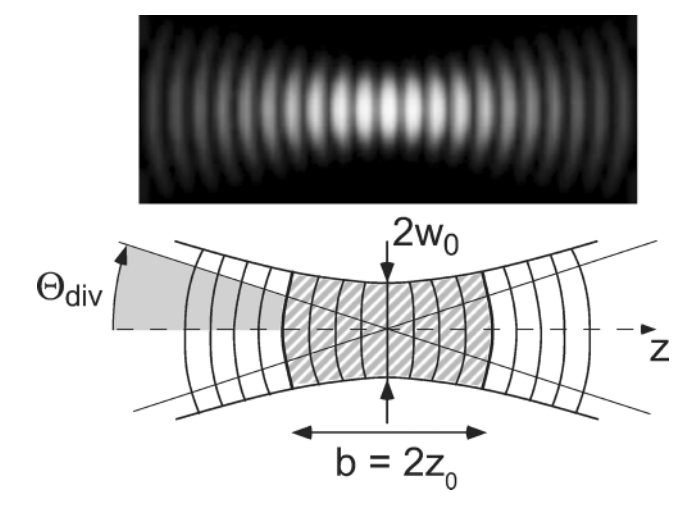
\includegraphics[width=0.8\linewidth]{figures/fabry-perot/gaussian-mode-near-beam-waist}
	\caption[A Gaussian beam near its beam waist.]
	{A Gaussian beam near its beam waist.
		Near the center they resemble plan wave fronts, while outside they converge towards spherical wave fronts.
		They Rayleighzone is shaded at the lower part of the figure.\cite{meschede_optik_2008}}
	\label{fig:gaussian-mode-near-beam-waist}
\end{figure}
For a proper description of a Gaussian beam as shown in figure~\ref{fig:gaussian-mode-near-beam-waist} the following  parameters have to be introduced
\begin{itemize}
	\item \textbf{Evolving radius of curvature} $R(z)$:
	\begin{equation}
	\label{eq:radius-wavefronts}
	R(z)=z(1+(z_0/z)^2)
	\end{equation}
	\item \textbf{Beam waist} $2\omega_0$:
	\begin{equation}
	\label{eq:beam-waist}
	\omega_0^2=\lambda z_0/\pi
	\end{equation}
\end{itemize}
The beam waist $2\omega_0$ or beam radius $\omega_0$ describes the smallest  beam cross section at $z=0$.
If the wave propagates inside a medium with the refractive index $n$, $\lambda$ has to be replaced with $\lambda/n$.
The cross section of the beam waist  is then $\omega_0^2=\lambda z_0/(\pi n)$.

A Gaussian beam can be completely characterized at every point $z$ on the beam axis either with the parameter couple $(\omega_0, z_0)$ or alternatively with the real and imaginary part of $q(z)$.
The parameters of the Gaussian beam are transformed by the ray transfer matrix
\begin{equation}
\label{eq:ABCD-rule}
q_{out}=\frac{A q_{in} + B}{C q_{in} + D}
\end{equation}
with the parameters $A, B, C, D$ determined by the optical element transforming the Gaussian beam described by $q_{in}$.

\subsection{Higher Gauss modes}
The wave equation~\eqref{eq:wave-equation} can be simplified by only allowing monochromatic waves with harmonic time dependence
\begin{equation}
\mathbf{E}(\mathbf{r},t) = \operatorname{Re}\left(\mathbf{E}(\mathbf{r})e^{-i\omega t}\right).
\end{equation}
With $\omega^2=c^2\mathbf{k}^2$, the \textit{Helmholtz equation} can be deduced, which only depends on the location \textbf{r}
\begin{equation}
\left(\nabla^2+\mathbf{k}^2\right)\mathbf{E}(\mathbf{r})=0.
\end{equation}
In favor of a formal treatment of the Gaussian modes, the Helmholtz equation is split into its transversal and longitudinal contributions,
\begin{equation}
\nabla^2+k^2=\frac{\partial^2}{\partial z^2} + \nabla_T^2+k^2
\quad\mathrm{with}\quad
\nabla_T^2=\frac{\partial}{\partial x^2}+\frac{\partial}{\partial y^2} \ .
\end{equation}
Additionally, the electric field $E$ of equation~\eqref{eq:e-field-after-fresnel-approximation} is inserted into the Helmholtz equation.
It is also assumed that the amplitude $A$ only changes slowly in the order of the wavelength,
\begin{equation}
\frac{\partial}{\partial z} A = A' \ll kA \ ,
\end{equation}
which allows the approximation
\begin{equation}
\frac{\partial^2}{\partial z^2} A e^{ik\rho^2 /(2z)} \frac{e^{ikz}}{kz} \simeq (2ikA'-k^2A)e^{ik\rho^2/(2z)}\frac{e^{ikz}}{kz} \ ,
\end{equation}
and results in the \textit{paraxial Helmholtz equation},
\begin{equation}
\left(\nabla_T^2+2ik\frac{\partial}{\partial z}\right)A(\rho, z) = 0.
\end{equation}
The fundamental solution is the TEM$_{00}$ mode in equation~\eqref{eq:fundamental-gaussian-mode}. Examples of higher modes can be found in figure~\ref{fig:gauss-modes-higher-order}.
\begin{figure}[H]
	\centering
	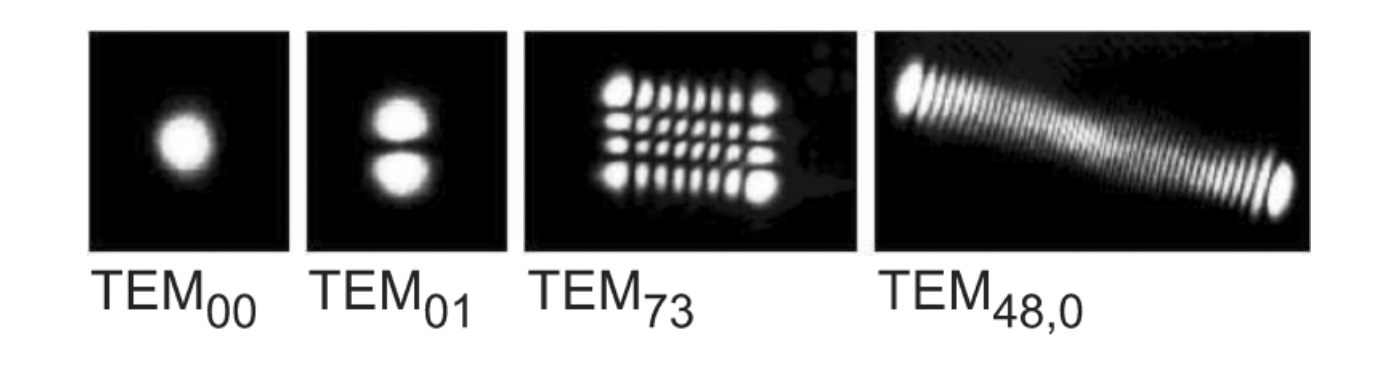
\includegraphics[width=0.9\linewidth]{figures/fabry-perot/gauss-modes-higher-order}
	\caption[Gaussian modes higher order of a simple Ti-sapphire laser]{Gaussian modes higher order of a simple Ti-sapphire laser.
		The asymmetry of the high modes are caused by technical inaccuracies of the resonator elements (mirrors, laser crystal).}
	\label{fig:gauss-modes-higher-order}
\end{figure}



\section{Fundamentals of Fabry-Pérot interferometers}


\subsection{Resonator losses}
For the following discussion of the \ac{FPI}, a two-mirror-resonator with the reflecting surfaces facing each other and air as medium in between is assumed.
The theoretical foundation is provided by the work of \textcite{ismail_fabry-perot_2016}.

The time the light needs for one roundtrip is given by
\begin{equation}
t_{RT} = \frac{2l}{c}
\end{equation}
where $l$ is the geometrical length of the resonator and $c$ is the speed of light in air.

The photon-decay time $\tau_c$ of the interferometer is then given by
\begin{equation}
\frac{1}{\tau_c} = - \frac{\ln(R_1 \cdot R_2)}{t_{RT}}
\end{equation}
where $R_1$ and $R_2$ are the corresponding intensity reflectivities of the mirrors.

The number of photons at frequency $\nu$ inside the resonator is described by the differential rate equation
\begin{equation}
\frac{d}{dt} \varphi(t) = - \frac{1}{\tau_c}\varphi(t).
\end{equation}
With a number $\varphi_s$ of photons at $t=0$ the integration gives
\begin{equation}
\label{eq:photon-decay}
\varphi(t)=\varphi_s e^{-t/\tau_c}
\end{equation}

\subsection{Resonance frequencies, free spectral range and spectral line shapes}
The round-trip phase shift at frequency $\nu$ is given by
\begin{equation}
\label{eq:round-trip-phase-shift-phi}
2 \phi(\nu) = 2 \pi \nu t_{RT} = 2 \pi \nu \frac{2l}{c}
\end{equation}
where $\phi(\nu)$ is the single-pass phase shift between the mirrors.

Resonances are visible for frequencies $\nu$ at which the light interferes constructively after one round trip.
Two adjacent resonance frequencies differ in their round trip phase shift by $2 \pi$.
Hence, the free spectral range $\Delta \nu_{FSR}$, the frequency difference between two adjacent resonance frequencies, can be calculated from equation~\eqref{eq:round-trip-phase-shift-phi}
\begin{align}
2\Delta\phi_{FSR} = 2\pi \\
\Rightarrow 2\pi\Delta\nu_{FSR}\frac{2l}{c} = 2\pi\\
\label{eq:free-spectral-range}
\Rightarrow \Delta\nu_{FSR} = \frac{c}{2l}
\end{align}

According to equation~\eqref{eq:photon-decay} the number of photons decays with the photon-decay time $\tau_c$.
With $E_{q,s}$ representing the initial amplitude, the electric field at $\nu_q$ is given by
\begin{equation}
E_q(t) =
\begin{cases}
E_{q,s} \cdot e^{i2\pi\nu_qt} \cdot e^{-t/(2\tau_c)} &  t \geq 0 \\
0 &  t < 0
\end{cases}
.
\end{equation}
The Fourier transformation of the electric field can be expressed as
\begin{equation}
\tilde{E}_q(\nu) = \int_{-\infty}^\infty E_q(t)e^{-i2\pi\nu t}dt = E_q(t) \int_{0}^\infty e^{.[1/(2\tau_c)+i2\pi(\nu-\nu_q)]t}dt = E_{q,s} \frac{1}{(2\tau_c)^{-1}+i2\pi(\nu-\nu_q)}.
\end{equation}
The normalized spectral line shape per unit frequency is then given by
\begin{align}
\label{eq:round-trip-phase-shift}
\tilde{\gamma_q}(\nu)&=\frac{1}{\tau_c}\left|\frac{\tilde{E}_q(\nu)}{E_{q,s}}\right|^2=\frac{1}{\tau_c}\left|\frac{1}{(2\tau_c)^{-1}+i2\pi(\nu-\nu_q)}\right|^2 = \frac{1}{\tau_c}\frac{1}{(2\tau_c)^{-2}+4\pi^2(\nu-\nu_q)^2} \\
&=\frac{1}{\pi}\frac{1/(4\pi\tau_c)}{1/(4\pi\tau_c)^2+(\nu-\nu_q)^2}
\end{align}
with $\int \tilde{\gamma_q}(\nu)d\nu=1$.

By defining the full-width-at-half-maximum linewidth (FWHM) $\Delta\nu_c$, $\tilde{\gamma_q}(\nu)$ can be obtained
\begin{equation}
\Delta \nu_c = \frac{1}{2\pi\tau_c} \Rightarrow \tilde{\gamma_q}(\nu) = \frac{1}{\pi}\frac{\Delta \nu_c/2}{\left(\Delta\nu_c/2\right)^2+\left(\nu-\nu_q\right)^2}.
\end{equation}
Afterwards the Cauchy lines are normalized so that the peak is at unity
\begin{equation}
\label{eq:cauchy}
\gamma_{q,L}(\nu)=\frac{\pi}{2}\Delta\nu_c\tilde{\gamma_q}(\nu)=\frac{(\Delta\nu_c)^2}{\left(\Delta \nu_c\right)^2+4\left(\nu-\nu_q\right)^2}
\end{equation}
with $\gamma_{q,L}(\nu_q)=1$.
\subsection{Airy distribution of Fabry-Pérot interferometers}

\begin{figure}[h]
	\centering
	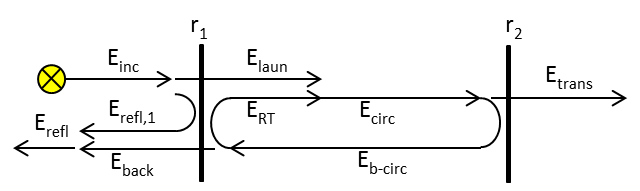
\includegraphics[width=0.7\linewidth]{figures/fabry-perot/Schematic_of_the_Fabry-Perot_interferometer}
	\caption[Fabry Pérot interferometer with electric field mirror reflectivities $r_1$ and $r_2$]{\ac{FPI} with electric field mirror reflectivities $r_1$ and $r_2$.
		Indicated in this figure are the electric fields resulting from an incoming $E_{inc}$, the reflected field $E_{refl,1}$ and transmitted field $E_{laun}$.
		$E_{circ}$ and $E_{circ,b}$ circulate inside the resonator, resulting in $E_{RT}$ after one round-trip. $E_{back}$ is the backwards transmitted field.\cite{noauthor_fabryperot_nodate}}
	\label{fig:schematicofthefabry-perotinterferometer}
\end{figure}
The response of the \ac{FPI} is calculated with the circulating-field approach~\cite{ismail_fabry-perot_2016}, where a steady-state is assumed.
$E_{circ}$ is the result of $E_{laun}$ interfering with $E_{RT}$.
$E_{laun}$ is the transmission of the incoming light $E_{inc}$ and $E_{RT}$ is $E_{circ}$ after one round-trip in the resonator, i.e., after the outcoupling losses of mirror 1 and 2.
Therefore, the field $E_{circ}$ can be calculated from $E_{launch}$ by
\begin{equation}
E_{circ} = E_{laun} + E_{RT} = E_{laun} + r_1 r_2 e^{-i 2 \phi} E_{circ} \Rightarrow \frac{E_{circ}}{E_{laun}} = \frac{1}{1 - r_1 r_2 e^{-i 2 \phi}}
\end{equation}
where $r_1$ and $r_2$ are the electric-field reflectivities of mirror 1 and 2.

The generic Cauchy distribution only considers light inside the mirrors and is defined as
\begin{equation}
A_{circ} = \frac{I_{circ}}{I_{laun}} = \frac{|E_{circ}|^2}{|E_{laun}|^2} = \frac{1}{\left|1 - r_1 r_2 e^{-i2\phi}\right|^2} = \frac{1}{\left(1-\sqrt{R_1 R_2}\right)^2 + 4\sqrt{R_1 R_2} \sin^2(\phi)}
\end{equation}
by using
\begin{align*}
\left|1-r_1 r_2 e^{-i2\phi}\right|^2 &= \left|1- r_1 r_2 \cos(2\phi) + i r_1 r_2 \sin(2\phi)\right|^2 = \left[1-r_1 r_2 \cos(2\phi)\right]^2 + r_1^2 r_2^2 \sin^2(2\phi) \\
 &=1+R_1 R_2 - 2\sqrt{R_1 R_2} \cos(2\phi) = \left(1-\sqrt{R_1 R_2}\right)^2 + 4 \sqrt{R_1 R_2} \sin^2(\phi)
\end{align*}
and additionally $R_i = r_i^2$ and $\cos(2\phi) = 1 -2\sin^2(\phi)$.

Commonly, light is sent through the \ac{FPI}. Therefore the following sections will use the Airy distribution $A'_{trans}$ described by
\begin{equation}
\label{eq:A-trans}
A'_{trans} = \frac{I_{trans}}{I_{inc}} = \frac{I_{circ} \cdot (1 - R_2)}{I_{laun} / (1 - R_1)} = (1-R_1)(1-R_2)A_{circ} = \frac{(1-R_1)(1-R_2)}{\left(1-\sqrt{R_1R_2}\right)^2+4\sqrt{R_1R_2}\sin^2(\phi)}
\end{equation}
with $\phi=\frac{\pi\nu}{\Delta \nu_{FSR}}$.

$A'_{trans}$ is displayed in figure~\ref{fig:airydistributionofafabry-perotinterferometer} for $R_1=R_2$. The peak value at one of its resonance frequencies calculates as follows
\begin{equation}
\max(A'_{trans}) = \frac{(1-R_1)(1-R_2)}{\left(1-\sqrt{R_1R_2}\right)^2} \stackrel{R_1=R_2}{=} 1.
\end{equation}

\begin{figure}[h]
	\centering
	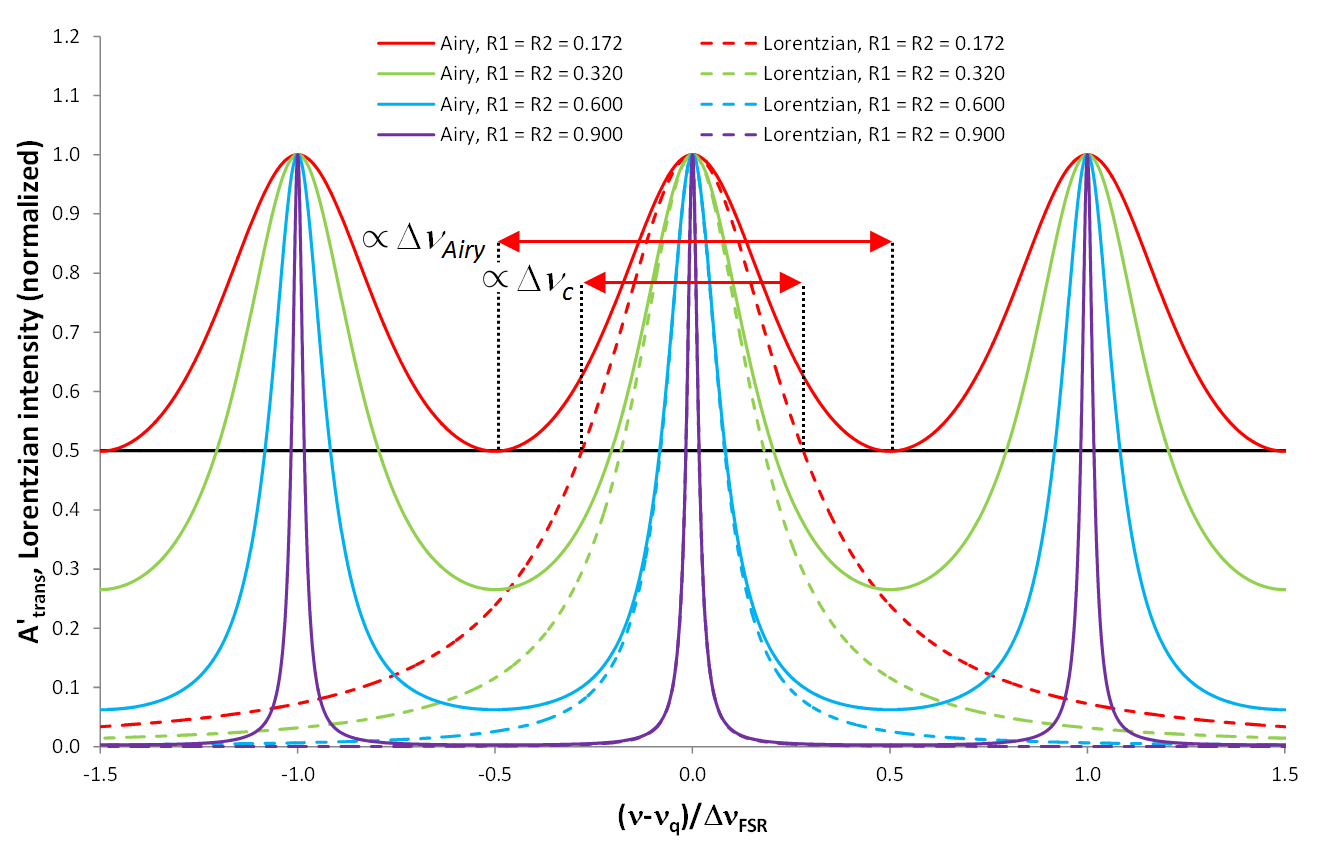
\includegraphics[width=0.8\linewidth]{figures/fabry-perot/Airy_distribution_of_a_Fabry-Perot_interferometer}
	\caption[Airy distribution $A'_{trans}$]{Airy distribution $A'_{trans}$ as described in equation~\eqref{eq:A-trans} compared to the Cauchy lines  $\gamma_{q,L}$ as described in equation~\eqref{eq:cauchy}~\cite{noauthor_fabryperot_nodate}.}
	\label{fig:airydistributionofafabry-perotinterferometer}
\end{figure}


\subsection{Airy linewidth and finesse}
The airy linewidth is defined as the \ac{FWHM} of $A'_{trans}$. It can be set in relation with the free spectral range $\Delta \nu_{FSR}$ and the mirror reflectivities as follows.

$A'_{trans}$ decreases to half of its peak value at $A'_{trans}(v_q) / 2$ when the phase shift $\phi$ changes by the amount $\Delta\phi$ so that the denominator of $A'_{trans}$ in equation~\eqref{eq:A-trans}  is twice as big
\begin{align}
\left(1-\sqrt{R_1R_2}\right)^2=4\sqrt{R_1R_2}\sin^2(\Delta\phi) \\
\label{eq:phase-shift-R}
\Rightarrow \Delta\phi=\arcsin\left(\frac{1-\sqrt{R_1R_2}}{2\sqrt[4]{R_1R_2}}\right)
\end{align}
With equation~\eqref{eq:round-trip-phase-shift-phi} and \eqref{eq:free-spectral-range}, the phase shift can be expressed as
\begin{align}
\phi &= \frac{\pi \nu}{\Delta \nu_{FSR}} \\
\label{eq:phase-shift-nu}
\Rightarrow \Delta \phi &= \frac{\pi (\Delta \nu_{Airy}/2)}{\Delta \nu_{FSR}}.
\end{align}
Therefore, with equation~\eqref{eq:phase-shift-R} and \eqref{eq:phase-shift-nu} the \ac{FWHM} linewidth is given by
\begin{equation}
\Delta \nu_{Airy} = \Delta \nu_{FSR}\frac{2}{\pi}\arcsin\left(\frac{1-\sqrt{R_1R_2}}{2\sqrt[4]{R_1R_2}}\right).
\end{equation}

The finesse of the Airy distribution of a \ac{FPI} is defined as
\begin{equation}
\label{eq:f-airy}
F_{Airy} := \frac{\Delta \nu_{FSR}}{\Delta \nu_{Airy}} = \frac{\pi}{2}\left[\arcsin\left(\frac{1-\sqrt{R_1R_2}}{2\sqrt[4]{R_1R_2}}\right)\right]^{-1}
\end{equation}
and is therefore only dependent on the mirror reflectivities $R_1$ and $R_2$.

\begin{figure}[H]
	\centering
	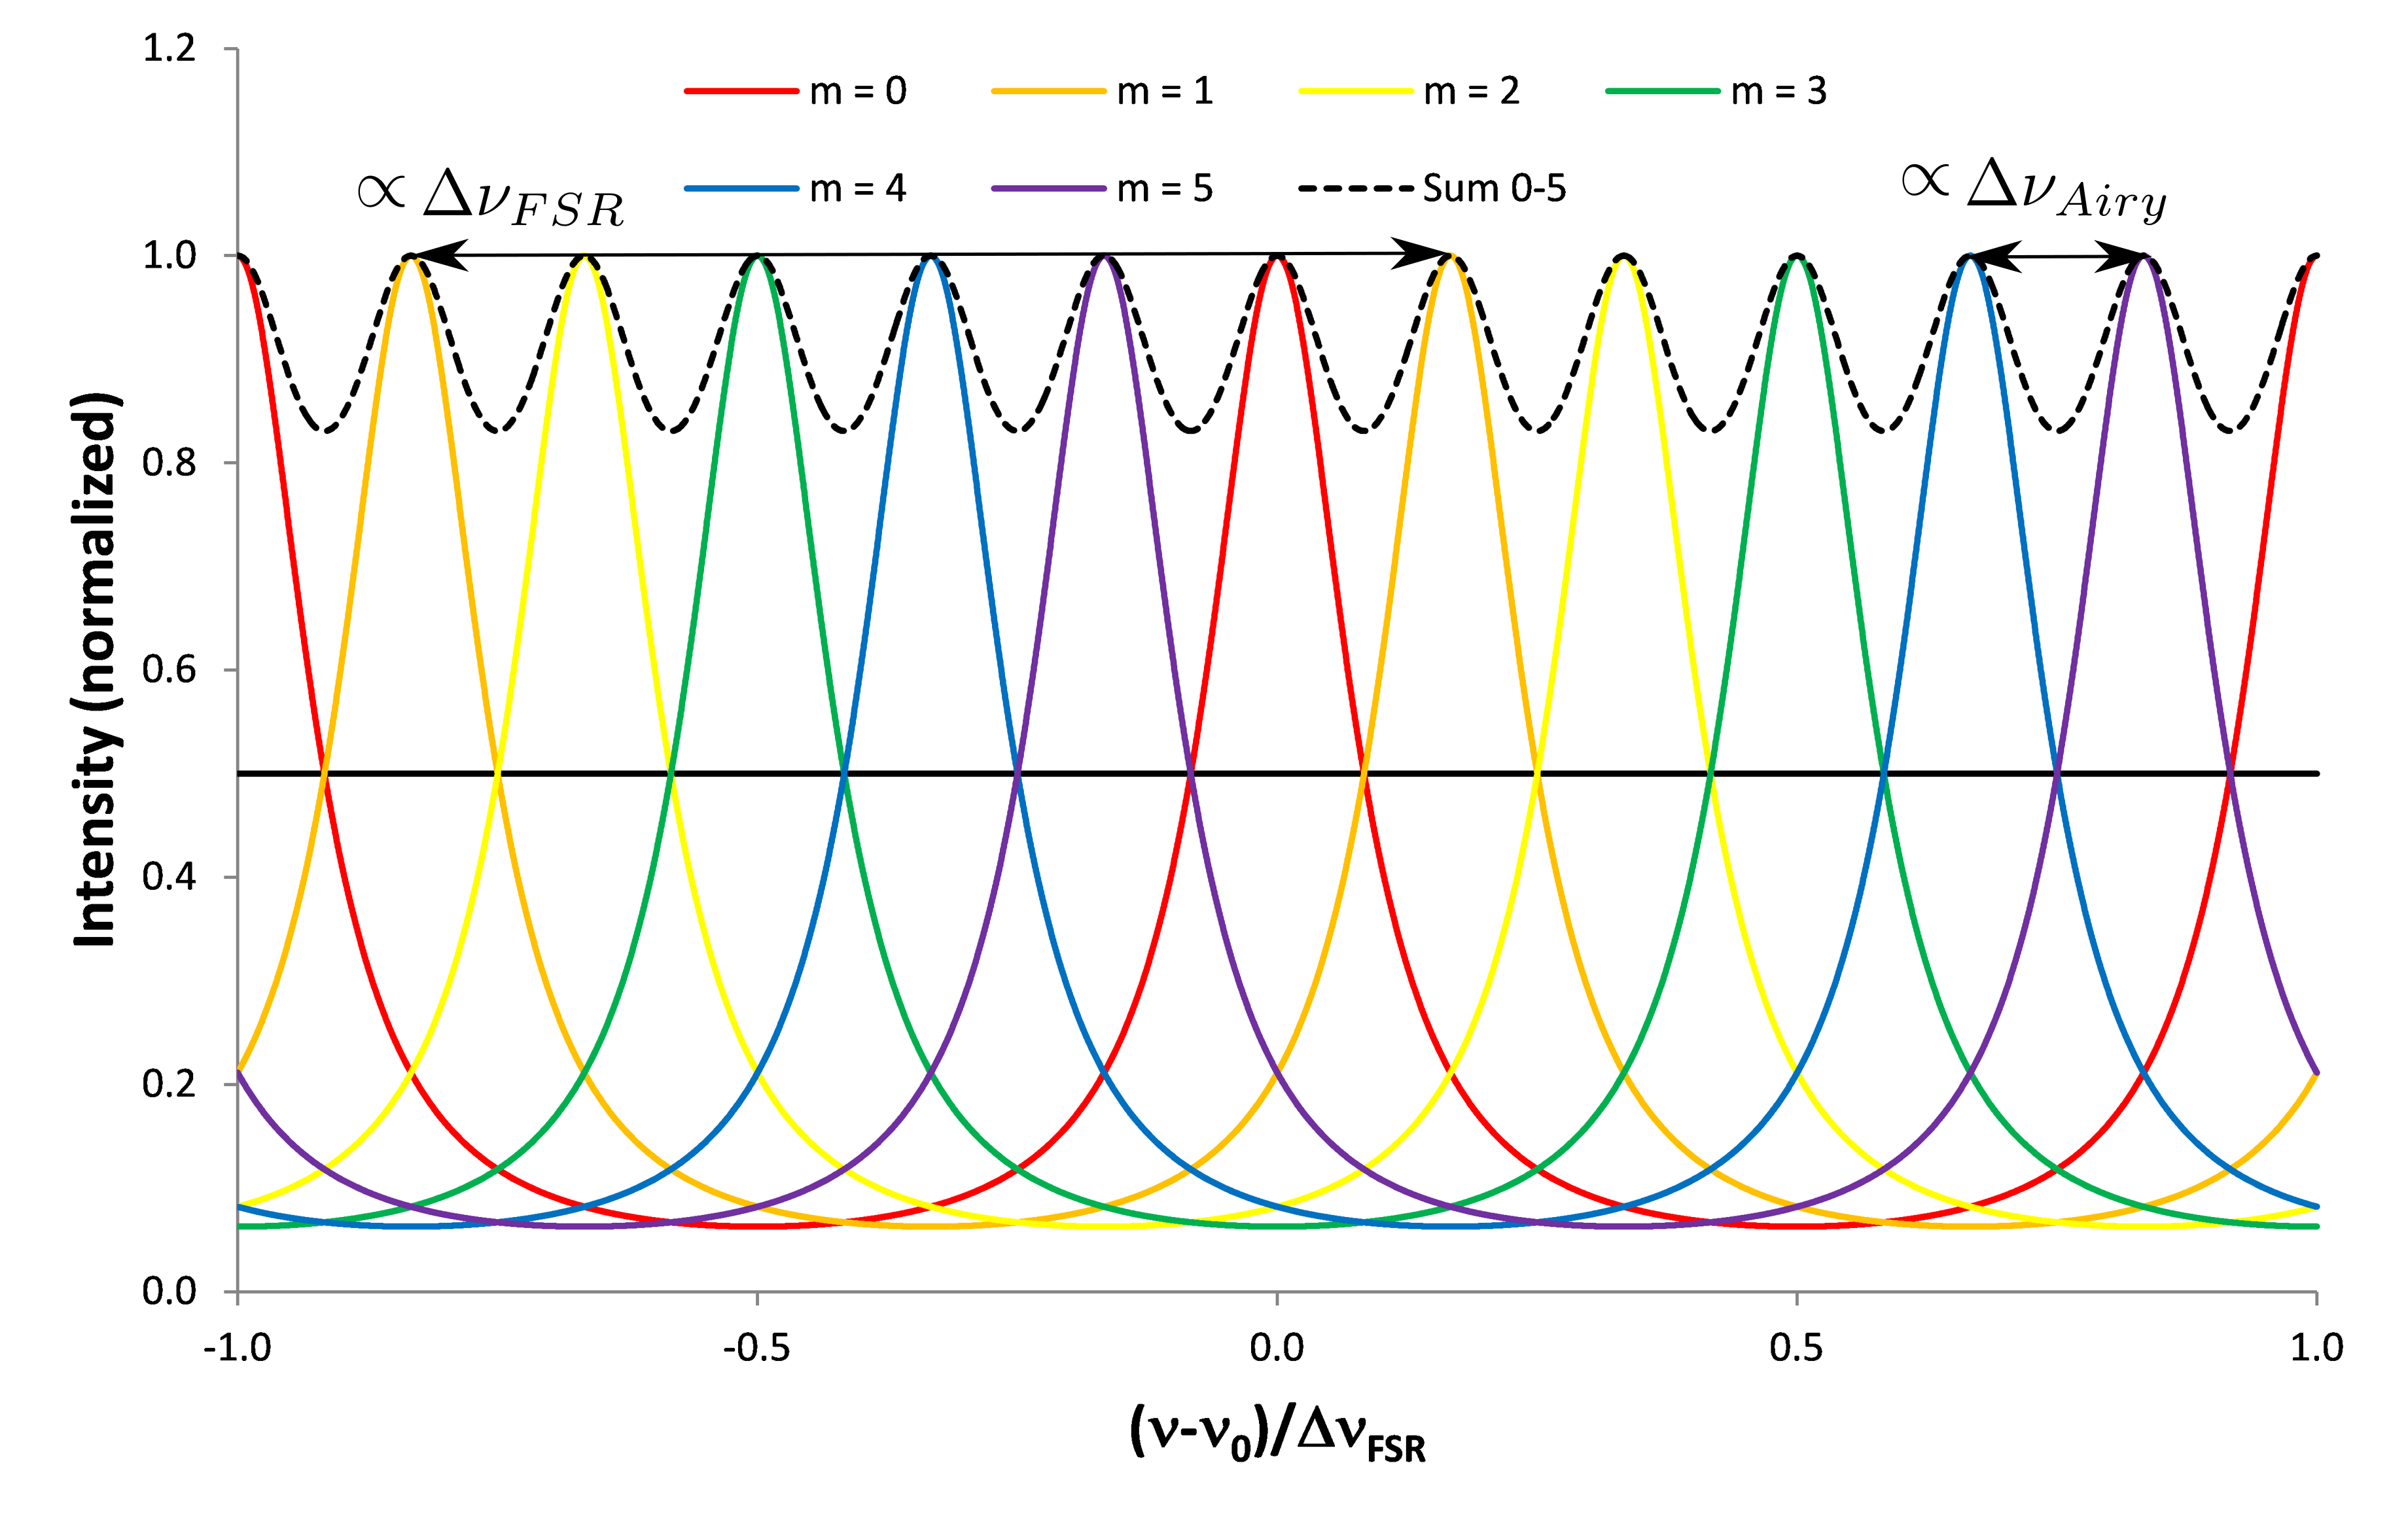
\includegraphics[width=0.8\linewidth]{figures/fabry-perot/Airy_finesse_of_a_Fabry-Perot_interferometer}
	\caption[Demonstration of the physical meaning of the Airy finesse $F_{Airy}$]{Demonstration of the physical meaning of the Airy finesse $F_{Airy}$.
		The coloured lines are Airy distributions created by light at distinct frequencies $\nu_m$, while scanning the resonator length. When the light occurs at frequencies $\nu_m = \nu_q+m\Delta \nu_{Airy}$, the adjacent Airy distributions are separated from each other by $\nu_{Airy}$, therefore fulfilling the Taylor criterion.
		Since in this example $F_{airy}=6$  exactly six peaks fit inside the free spectral range.
		As can be seen in the figure the Airy finesse $F_{Airy}$ quantifies the maximum number of peaks that can be resolved ~\cite{noauthor_fabryperot_nodate}.}
	\label{fig:airyfinesseofafabry-perotinterferometer}
\end{figure}


The Airy finesse is the determining property when it comes to the spectral resolution of the \ac{FPI}. This can be made visible by comparing its message with the Taylor criterion for the resolution of two adjacent peaks.
The Taylor criterion proposes that two spectral lines are resolvable when the separation of the maxima is greater than the \ac{FWHM}.
As displayed in figure~\ref{fig:airyfinesseofafabry-perotinterferometer}, the Airy finesse is equal to the number of Airy distributions originating from light at certain frequencies $\nu_m$ which do not overlap at a point higher than half of their maxima.
Hence, the Airy finesse describes the spectral resolution in a way that is consistent with the Taylor criterion.



\subsection{Mode matching and spatial filtering}
\label{subsec:mode-matching-spatial-filtering}
One fundamental challenge of Fabry Pérot interferometry is how to efficiently couple an incident beam of light into a given mode of the resonator.
The following discussion is based on the work of \textcite{yariv_photonics:_2007} and \textcite{meschede_optik_2008}.
\begin{figure}[H]
	\centering
	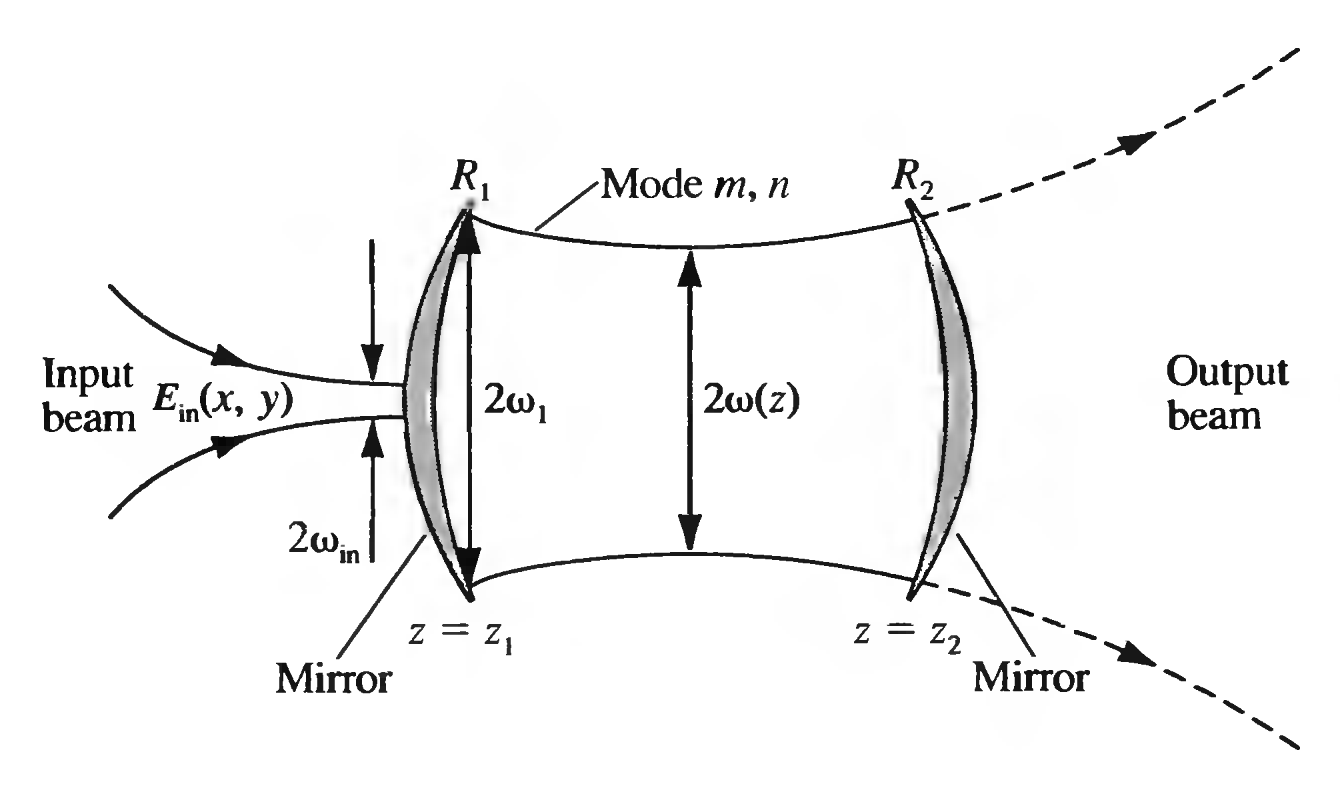
\includegraphics[width=0.7\linewidth]{figures/fabry-perot/excitation-of-transverse-mode}
	\caption{Incident monochromatic beam of light exciting transverse mode $m$, $n$ of a resonator~\cite{yariv_photonics:_2007}}
	\label{fig:excitation-of-transverse-mode}
\end{figure}

In sketched with figure~\ref{fig:excitation-of-transverse-mode}, an input beam $E_{in}$ propagates into the resonator and potentially excite its modes $E_{mn}(x,y)$, where $m$, $n$ are the transverse mode integers of the Gaussian beam of the optical resonator.
Since $E_{mn}(x,y)$ describes a complete orthogonal set of wavefunctions they satisfy
\begin{equation}
\label{eq:complete-set-mn-modes}
\iint E_{mn}(x,y) E^*_{m'n'}(x,y) dx dy = 0 \quad \mathrm{unless} \ m=m' \ \mathrm{and} \ n=n'.
\end{equation}
and
\begin{equation}
\label{eq:superposition-mn-modes}
E_{in}(x,y) = \sum_{mn}a_{mn}E_{mn}(x,y)
\end{equation}
where $a_{mn}$ are constants.
By multiplying both sides of equation~\eqref{eq:superposition-mn-modes} with $E_{mn}^*$, integrating over the whole $x$-$y$-plane and using equation~\eqref{eq:complete-set-mn-modes}, the following expression can be obtained
\begin{equation}
\label{eq:a-mn}
a_{mn}=\frac{\iint E_{in}(x,y)E^*_{mn}(x,y) dx dy}{\iint E_{mn}(x,y)E^*_{mn}(x,y) dx dy}
\end{equation}
The efficiency of coupling an incident field into a spatial mode $E_{mn}$ is defined as
\begin{equation}
\label{eq:coupling-efficiency-first}
\eta_{mn}=\frac{\textrm{Power coupled into mode } mn}{\textrm{Total incident power}}=
\frac{\iint \left|a_{mn} E_{mn}(x,y)\right|^2 dx dy}{\iint \left|E_{in}(x,y)\right|^2 dx dy}.
\end{equation}
By inserting equation~\eqref{eq:a-mn} into equation~\eqref{eq:coupling-efficiency-first} the following expression can be obtained
\begin{equation}
\label{eq:coupling-efficiency-second}
\eta_{mn}= \frac{\left|\iint E_{in}(x,y)E^*_{mn}(x,y) dx dy\right|^2}{\iint \left|E_{in}(x,y)\right|^2 dx dy \cdot \iint \left|E_{mn}(x,y)\right|^2 dx dy}.
\end{equation}
From equation~\eqref{eq:coupling-efficiency-second} can be deduced that for an input beam with the \textit{same} spatial dependency as the mode to be excited
\begin{equation}
E_{in}(x,y) \sim E_{mn}(x,y)
\end{equation}
all of the incident power goes into $E_{mn}$, i.e. $\eta_{mn}=1$ and all other $\eta_{m'n'}$ are zero.
Usually, the fundamental TEM$_{00}$ mode is desired and equation~\eqref{eq:coupling-efficiency-second} implies that a pure Gaussian beam excites only the fundamental mode and the interferometer will then irradiate a pure Gaussian beam as well.
In practise, additional measures are necessary such as matching the radius of curvature by Gaussian beam focusing.

\begin{figure}[h]
	\centering
	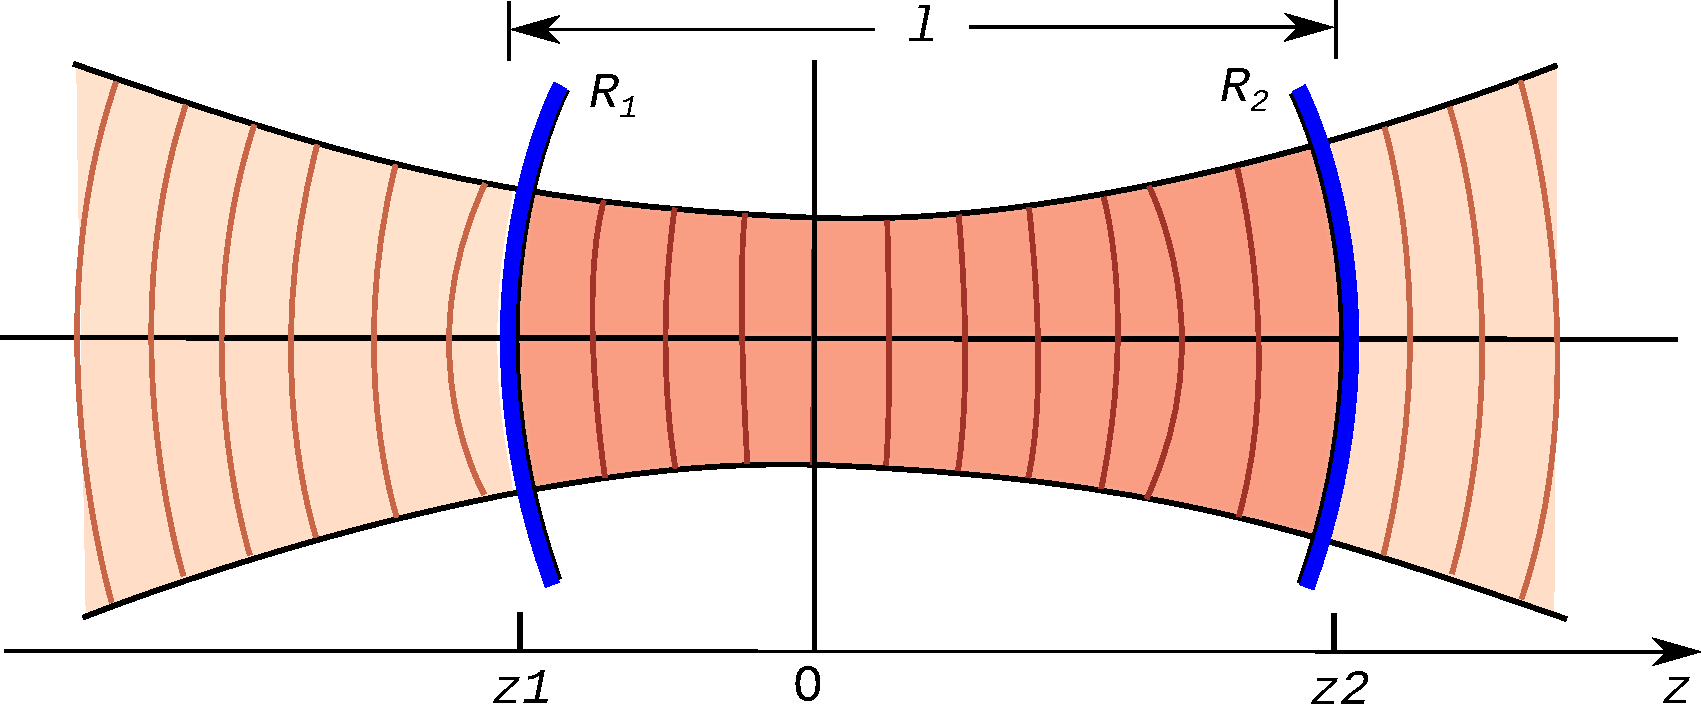
\includegraphics[width=0.8\linewidth]{figures/fabry-perot/gaussian-beam-focusing}
	\caption[Mode matching of an Gaussian beam into a Fabry Pérot interferometer.]
	{Mode matching of an Gaussian beam into a Fabry Pérot interferometer.
		Incoming Gaussian beam described by $q_{in}$ transformed by a lens into a Gaussian beam described by $q_{out}$.
		The parameters $b_1$ and $b_2$ describe the radii of the two mirrors.}
	\label{fig:gaussian-beam-focusing}
\end{figure}

In order to match the radius of curvature of the incoming Gaussian beam with the radius of curvature of the resonator a lens is inserted as depicted in figure~\ref{fig:gaussian-beam-focusing}. Light with a beam waist of $\omega_{01}$ gets focused into the resonator. Transformations by thin lenses can be described with the ray transfer matrix introduced in subsection~\ref{subsec:gaussian-beam}:
\begin{equation}
\begin{pmatrix}
A & B \\
C & D
\end{pmatrix}
=
\begin{pmatrix}
1 & 0 \\
\frac{-1}{f} & 1
\end{pmatrix}
\end{equation}
with $f$ as the wavelength of the lens.
The incoming beam described by $q_{in}$ is transformed by the lens into a beam described by $q_{out}$ according to equation~\eqref{eq:beam-waist} and \eqref{eq:ABCD-rule}
\begin{equation}
q_{in} = z + i \frac{\pi n \omega_{0,in}^2}{\lambda} \qquad \mathrm{and} \qquad
q_{out} = \frac{q_{in}}{q_{in} \cdot \frac{-1}{f} + 1} =  z + i \frac{\pi n \omega_{0,out}^2}{\lambda}
\end{equation}
with $n\approx 1$ for air. Together with equation~\eqref{eq:beam-waist} to following relation can be deduced
\begin{equation}
\label{eq:w-o-out}
\omega_{0,out}^2 = \frac{\omega_{0,in}^2}{\left(1-\frac{z}{f}\right)^2+\left(\frac{\pi \omega_{0,in}}{\lambda f}\right)^2}.
\end{equation}
The radii of curvature have to match.
For given mirrors (described by $R_{mirror}$) and lens (described by $f$) the input beam waist has to be adjusted according to equation~\eqref{eq:radius-wavefronts} and \eqref{eq:beam-waist}
\begin{align}
R_{mirror} \stackrel{!}{=} R_{gauss}(z= l/2)\\
R_{mirror} \stackrel{!}{=} \frac{l}{2} \left(1+\left(\frac{2z_{0,out}}{l}\right)^2\right) \\
\label{eq:R-mirror-1}
R_{mirror} \stackrel{!}{=} \frac{l}{2} \left(1+\left(\frac{2\omega_{0,out}^2 \pi}{l \lambda}\right)^2\right).
\end{align}
Inserting equation~\eqref{eq:R-mirror-1} into equation~\eqref{eq:w-o-out} results in the condition for mode matching
\begin{equation}
\label{eq:R-mirror-2}
R_{mirror} = \frac{l}{2} \left(1+\left(\frac{2 \omega_{0,in}^2 \pi}{\left(\left(1-\frac{z}{f}\right)^2+\left(\frac{\pi \omega_{0,in}}{\lambda f}\right)^2\right)l \lambda}\right)^2\right).
\end{equation}

One way to further suppress higher modes is \textit{spatial filtering}. It can be seen in figure~\ref{fig:gauss-modes-higher-order} that the effective area of a mode increases with its order $(m, n)$. Figure~\ref{fig:spatial-filtering-of-gauss-modes} shows one way to suppress higher modes consisting of a focusing lens and a pin hole which diameter matches the one of the TEM$_{00}$ mode.

\begin{figure}[H]
	\centering
	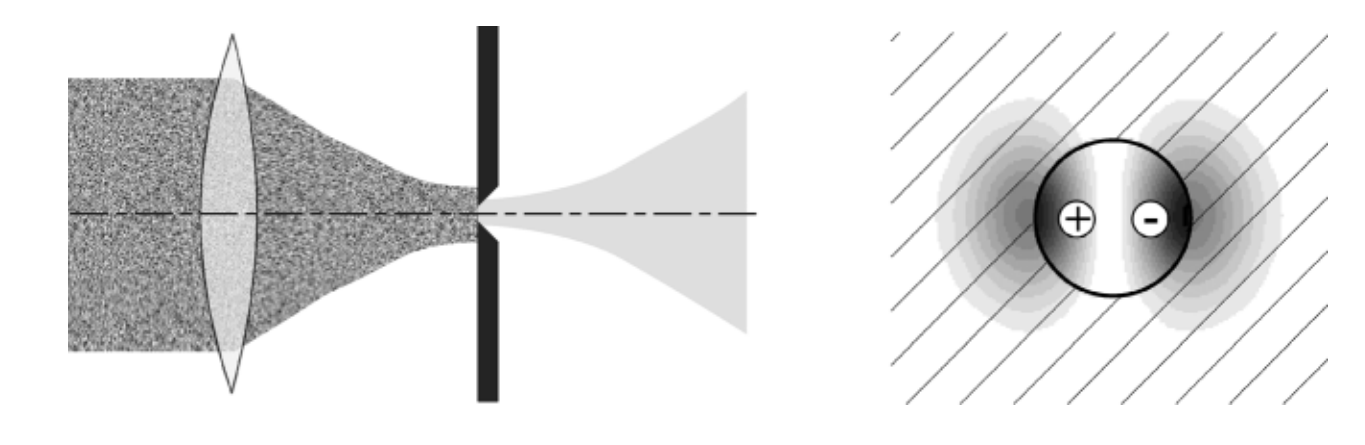
\includegraphics[width=0.8\linewidth]{figures/fabry-perot/spatial-filtering-of-gauss-modes}
	\caption[Spatial filtering of Gauss modes.]{Spatial filtering of Gauss modes.
		In front of the aperture, the beam consists of a superposition of multiple Gauss modes.
		In the example of TEM$_{01}$ is displayed how higher modes are suppressed by the aperture.~\cite{meschede_optik_2008}}
		\label{fig:spatial-filtering-of-gauss-modes}
	\end{figure}



\subsection{Confocal setup}
\label{subsec:confocal-setup}

If the incoming beam would represent a perfect TEM$_{00}$ mode, spatial filtering would not be necessary and mode matching would not have to be done as precise.
Unfortunately, this can not always be guaranteed and counteractions like mode matching and spatial filtering discussed in subsection~\ref{subsec:mode-matching-spatial-filtering} are tedious and error prone.
Arranging the mirrors of an \ac{FPI} into a confocal arrangement reduces the need for these measures.
By giving up the ability to choose different free spectral ranges with a given pair of mirrors, the confocal setup liberates from mode matching considerations as the cavity is mode degenerated, i.e. the frequency of certain axial and transverse cavity modes are the same.
The following discussion is based on the work of \textcite{hercher_spherical_1968}.

A quasi-monochromatic beam of wavelength $\lambda_0$ is composed of transverse modes TEM$_{\textrm{mnq}}$, where the subscripts $m$ and $n$ denote the amplitude distribution of the normal mode on a surface of constant phase and $q$ the number of axial modes inside the resonator.
Each of these modes resonates for mirror separations satisfying
\begin{equation}
l = \frac{\lambda_0}{2}\{q + \left(1 + m + n\right) \cos^{-1}\left[(1-l/b_1)(1-l/b_2)\right]^{1/2}\}
\end{equation}
where the parameters $b_1$ and $b_2$ describe the radii of the two mirrors as can be seen in figure~\ref{fig:gaussian-beam-focusing}.

For the confocal setup $l=b_1=b_2$ justifies the approximation
\begin{equation}
l \approx \frac{\lambda_0}{2} \left[q + \left(1+m+n\right)\right].
\end{equation}
The modes resonate at mirror separations of either
\begin{align}
l = \frac{\lambda_0}{2}(p+1) \qquad p&\in\mathbb{N} \textrm{ and } (m+n) \textrm{ even,} \\
l = \frac{\lambda_0}{2}(p) \qquad p&\in\mathbb{N} \textrm{ and } (m+n) \textrm{ odd.}
\end{align}
If mode matching is not executed, it can be assumed that the incoming beam consists of an approximately equal number of even and odd transverse modes.
The resonance cavity length $l$ does not depend on $n$,$m$ and $q$ anymore but only on one integer $p$. The transversal modes are degenerate and fulfil
\begin{equation}
\label{eq:confocal-degenerate}
l = \frac{\lambda_0 p}{2}.
\end{equation}
It can be additionally concluded from equation~\eqref{eq:confocal-degenerate} that a change of $\lambda_0/2$ in the mirror separation scans through one free spectral range.
\section{Simulation}

The goal in building up a scanning \ac{FPI} is to resolve features of the emission spectra of GaAs \aclp{QD} described in chapter~\ref{chapter:quantum-dot}.
More precisely, it is intended to resolve the shape of the \ac{ZPL} and the \ac{PSB}.
Equation~\ref{eq:f-airy} shows that the finesse is constant for a given pair of mirrors.
If the spectrum to be resolved is broad, a higher free spectral range $\Delta \nu_{FSR}$ has to be chosen, under the loss of resolution.
If the spectrum contains fine details which need to be resolved, a lower $\nu_{Airy}$ has to be chosen, which results in a lower free spectral range $\Delta \nu_{FSR}$.
Hence, the thin \ac{ZPL} and the broad \ac{PSB} can not be resolved with the same setup.
Instead, the mirror distances have to be adjusted and in the confocal setup discussed in subsection~\ref{subsec:confocal-setup} the mirrors have to be changed as well.

The zero-phonon line is described with a Cauchy distribution
\begin{equation}
\Phi_{ZPL}(\lambda) = \frac{1}{\pi \cdot \Delta\lambda_{ZPL} \cdot 0.5 \left[1+\left(\frac{\lambda - \lambda_{0, ZPL}}{\Delta\lambda_{ZPL} \cdot 0.5}\right)^2\right]}
\end{equation}
with $\lambda_{0, zero}$ as the center wavelength and $\Delta\lambda_{ZPL}$ as the spectral range of the zero-phonon line which can be found in table~\ref{tab:quantum-dot-emission}.

The phonon side band is described with a Gauss distribution
\begin{equation}
\Phi_{PSB}(\lambda) = \frac{1}{\sqrt{2\cdot\pi\cdot \Delta\lambda_{PSB}^2}}\cdot exp\left(-\frac{(\lambda - \lambda_{0, PSB})^2}{2\cdot \Delta\lambda_{PSB}^2}\right)
\end{equation}
with $\lambda_{0, PSB}$ as the center wavelength and $\Delta\lambda_{PSB}$ as the spectral range of the phonon side band which can be found in table~\ref{tab:quantum-dot-emission} as well.

Together they describe the excitonic emission of the \ac{QD}
\begin{equation}
\Phi_{dot}(\lambda) = \Phi_{ZPL}(\lambda) + \Phi_{PSB}(\lambda)
\end{equation}
depicted in figure~\ref{fig:quantumdotemissionwavelengthenergy}.

\begin{figure}[H]
	\centering
	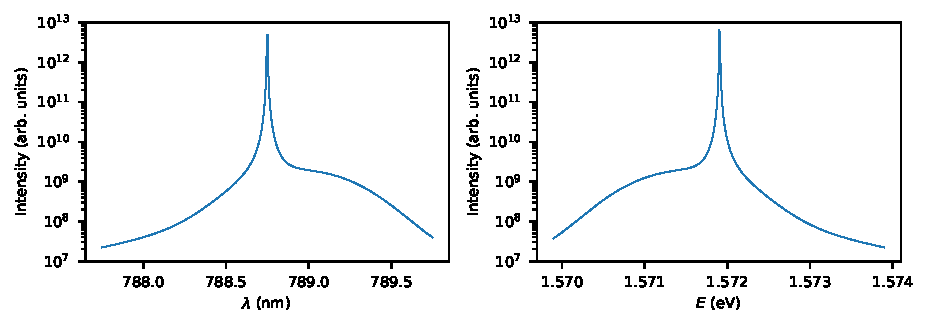
\includegraphics{figures/fabry-perot/plots/quantum_dot_emission_wavelength_energy}
	\caption[Simulated exciton emission of a GaAs quantum dot]{Simulated exciton emission of a GaAs quantum dot plotted dependant on (a) the wavelength $\lambda$ or (b) the energy $E$.
		The parameters can be found in table~\ref{tab:quantum-dot-emission}.}
	\label{fig:quantumdotemissionwavelengthenergy}
\end{figure}

$\Phi_{dot}(E)$ is transmitted through the \ac{FPI}.
As discussed the mirror distance $l$ is adjusted to a value which depends if a resolved \ac{ZPL} or a resolved \ac{PSB} is desired.
A comparison of the \ac{FPI} transmission $A'_{trans}(E)$ described in equation~\ref{eq:A-trans} with $R_1=R_2=\SI{98}{\percent}$ and $\Phi_{dot}(E)$ is shown in figure~\ref{fig:simulation-comparison-dot-fabry-perot-modes}.
\begin{figure}[H]
	\centering
	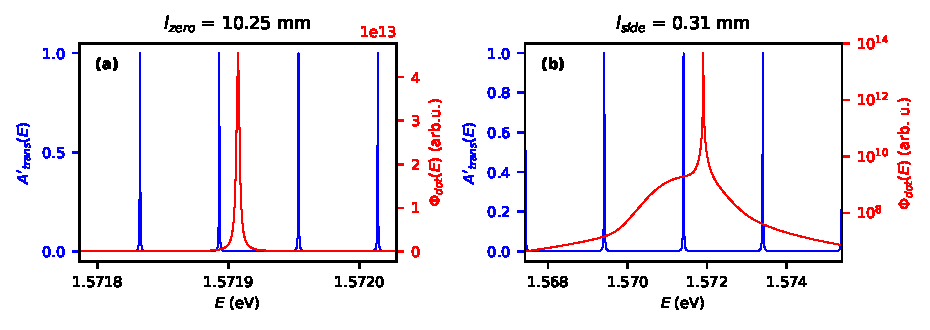
\includegraphics[width=\linewidth]{figures/fabry-perot/plots/simulation-comparison-dot-fabry-perot-modes}
	\caption{Transmission of the FPI modes $A'_{trans}$ compared to the exciton emission $\Phi_{dot}(E)$ for (a) ZPL and (b) PSB.}
	\label{fig:simulation-comparison-dot-fabry-perot-modes}
\end{figure}

The \ac{FPI} scans by continuously varying the mirror distance $l$ with a certain stepsize $\Delta l$ and measuring the output-photon-flux every time.
This process is sketched in figure~\ref{fig:simulation-comparison-dot-fabry-perot-sweep}.

\begin{figure}[H]
	\centering
	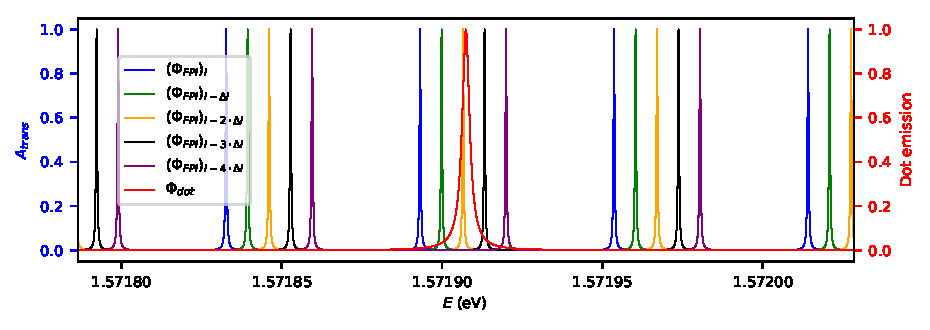
\includegraphics[width=\linewidth]{figures/fabry-perot/plots/simulation-comparison-dot-fabry-perot-sweep}
	\caption{Transmissions of the FPI modes $A'_{trans}$ (blue) for different mirror distances $l - m \cdot \Delta l$ with $m \in \mathbb{N}$ compared to the exciton emission $\Phi_{dot}(E)$ (red).}
	\label{fig:simulation-comparison-dot-fabry-perot-sweep}
\end{figure}


The unnormalized output-photon-flux of the scanning \ac{FPI} is then described with the convolution of $\Phi_{dot}(E)$ and $A'_{trans}(E)$
\begin{equation}
\tilde{\Phi}_{FPI}(E) = \int^{E_0 + n \cdot \Delta}_{E_0 - n  \cdot \Delta}  \Phi_{dot}(E')A'_{trans}(E - E') dE'
\end{equation}
with $E_0$ as the central energy of the exciton emission line, $\Delta$ as the free spectral range and $2n=4$ as the number of airy peaks considered for the numerical convolution.

\begin{figure}[H]
	\centering
	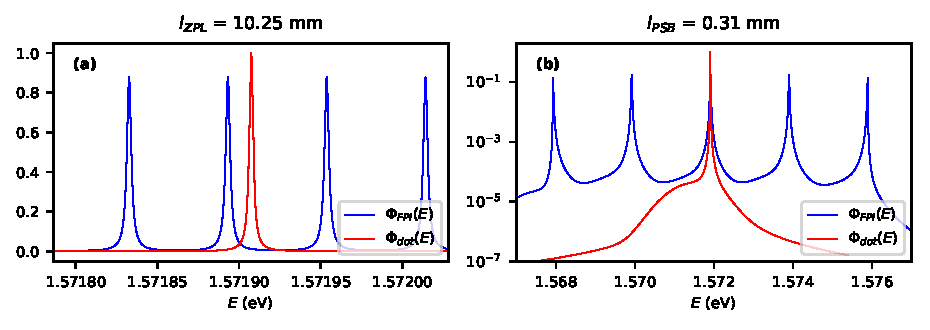
\includegraphics[width=\linewidth]{figures/fabry-perot/plots/simulation-comparison-dot-fabry-perot-output}
	\caption{Output-photon-flux of the scanning FPI $\Phi_{FPI}(E)$ (blue) compared to the exciton emission $\Phi_{dot}(E)$ (red) for (a) ZPl and (b) PSB.}
	\label{fig:simulation-comparison-dot-fabry-perot-output}
\end{figure}

$\tilde{\Phi}_{FPI}(E)$ can then be normalized with the integral of $A'_{trans}(E)$ over the same range
\begin{equation}
\Phi_{FPI}(E) =\frac{\tilde{\Phi}_{FPI}(E)}{\int^{E_0 + n \cdot \Delta}_{E_0 - n \cdot \Delta} A'_{trans}(E) dE}
\end{equation}
A comparison of $\Phi_{FPI}(E)$ and $\Phi_{dot}(E)$ is shown in figure~\ref{fig:simulation-comparison-dot-fabry-perot-output}.


From now on, only the \ac{ZPL}-path is shown as no new information is gained by examining both.
In order to estimate the accuracy of the scanning \ac{FPI}, the \ac{FPI} modes are shifted by $\Delta E$ in order to overlap with $\Phi_{dot}(E)$ as depicted in figure~\ref{fig:simulation-comparison-dot-fabry-perot-output-error}(a)
\begin{equation}
\overline{\Phi}_{FPI}(E) = \Phi_{FPI}(E - \Delta E).
\end{equation}
Afterwards, the absolute difference between those two $|\Phi_{dot}(E) - \Phi_{FPI}(E-\Delta E)|$ is calculated as shown in figure~\ref{fig:simulation-comparison-dot-fabry-perot-output-error}(b).
Now the relative error of  $\Phi_{fabry,perot}(E)$  for the given parameters and compared to the actual excitonic \ac{QD} emission  can be calculated
\begin{equation}
\epsilon = \frac{\int^{E_0 + \Delta / 2}_{E_0 - \Delta / 2} \left|\overline{\Phi}_{\text{FPI}}(E) - \Phi_{\text{dot}}(E)\right| dE }{\int^{E_0 + \Delta / 2}_{E_0 - \Delta / 2} \Phi_{\text{dot}}(E) dE}
\end{equation}
For the parameters in the \ac{ZPL} path this gives $\epsilon_{ZPL}=\SI{10.57}{\percent}$.


\begin{figure}[H]
	\centering
	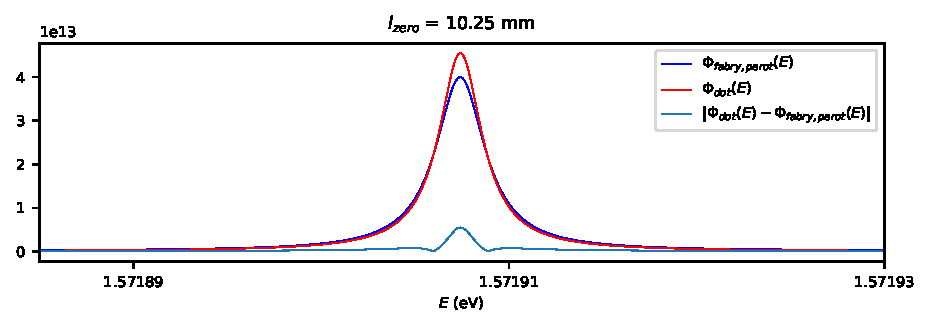
\includegraphics[width=\linewidth]{figures/fabry-perot/plots/simulation-comparison-dot-fabry-perot-output-error}
	\caption{In (a) the shifted output-photon-flux of the scanning FPI $\overline{\Phi}_{FPI}(E)$ (blue) compared to the exciton emission $\Phi_{dot}(E)$ (red) is displayed.
	In (b) the absolute difference between those two $ \left|\overline{\Phi}_{\text{FPI}}(E) - \Phi_{\text{dot}}(E)\right|$ (light blue) is additionally shown.}
	\label{fig:simulation-comparison-dot-fabry-perot-output-error}
\end{figure}


\newpage


\section{Setup and measurement}

Multiple \ac{FPI} setups were built up in order to test their suitability to resolve \ac{QD} emission.
The first version featured planar mirrors, while their distance was coarsely tunable with an adjustable platform and finely tunable with a piezoelectrical actuator.
However this setup with planar mirrors proved to be highly unstable and was therefore discarded.
The second version used smaller, planar-convex mirrors and a ground plate made of molybdenum.
This resulted in a stable \ac{FPI} which was also adjustable for various free-spectral ranges.
The measurements discussed in section~\ref{sec:fabry-measurements} are obtained with this setup.
However, the effort needed to mode-match for every measurement is too large to actually use it in further experiments.
That is why the confocal setup will be used in the future, even though the freedom to adjust the free-spectral range is lost.

\subsection{Scanning mode with fast photodiodes}

\begin{figure}[H]
	\centering
	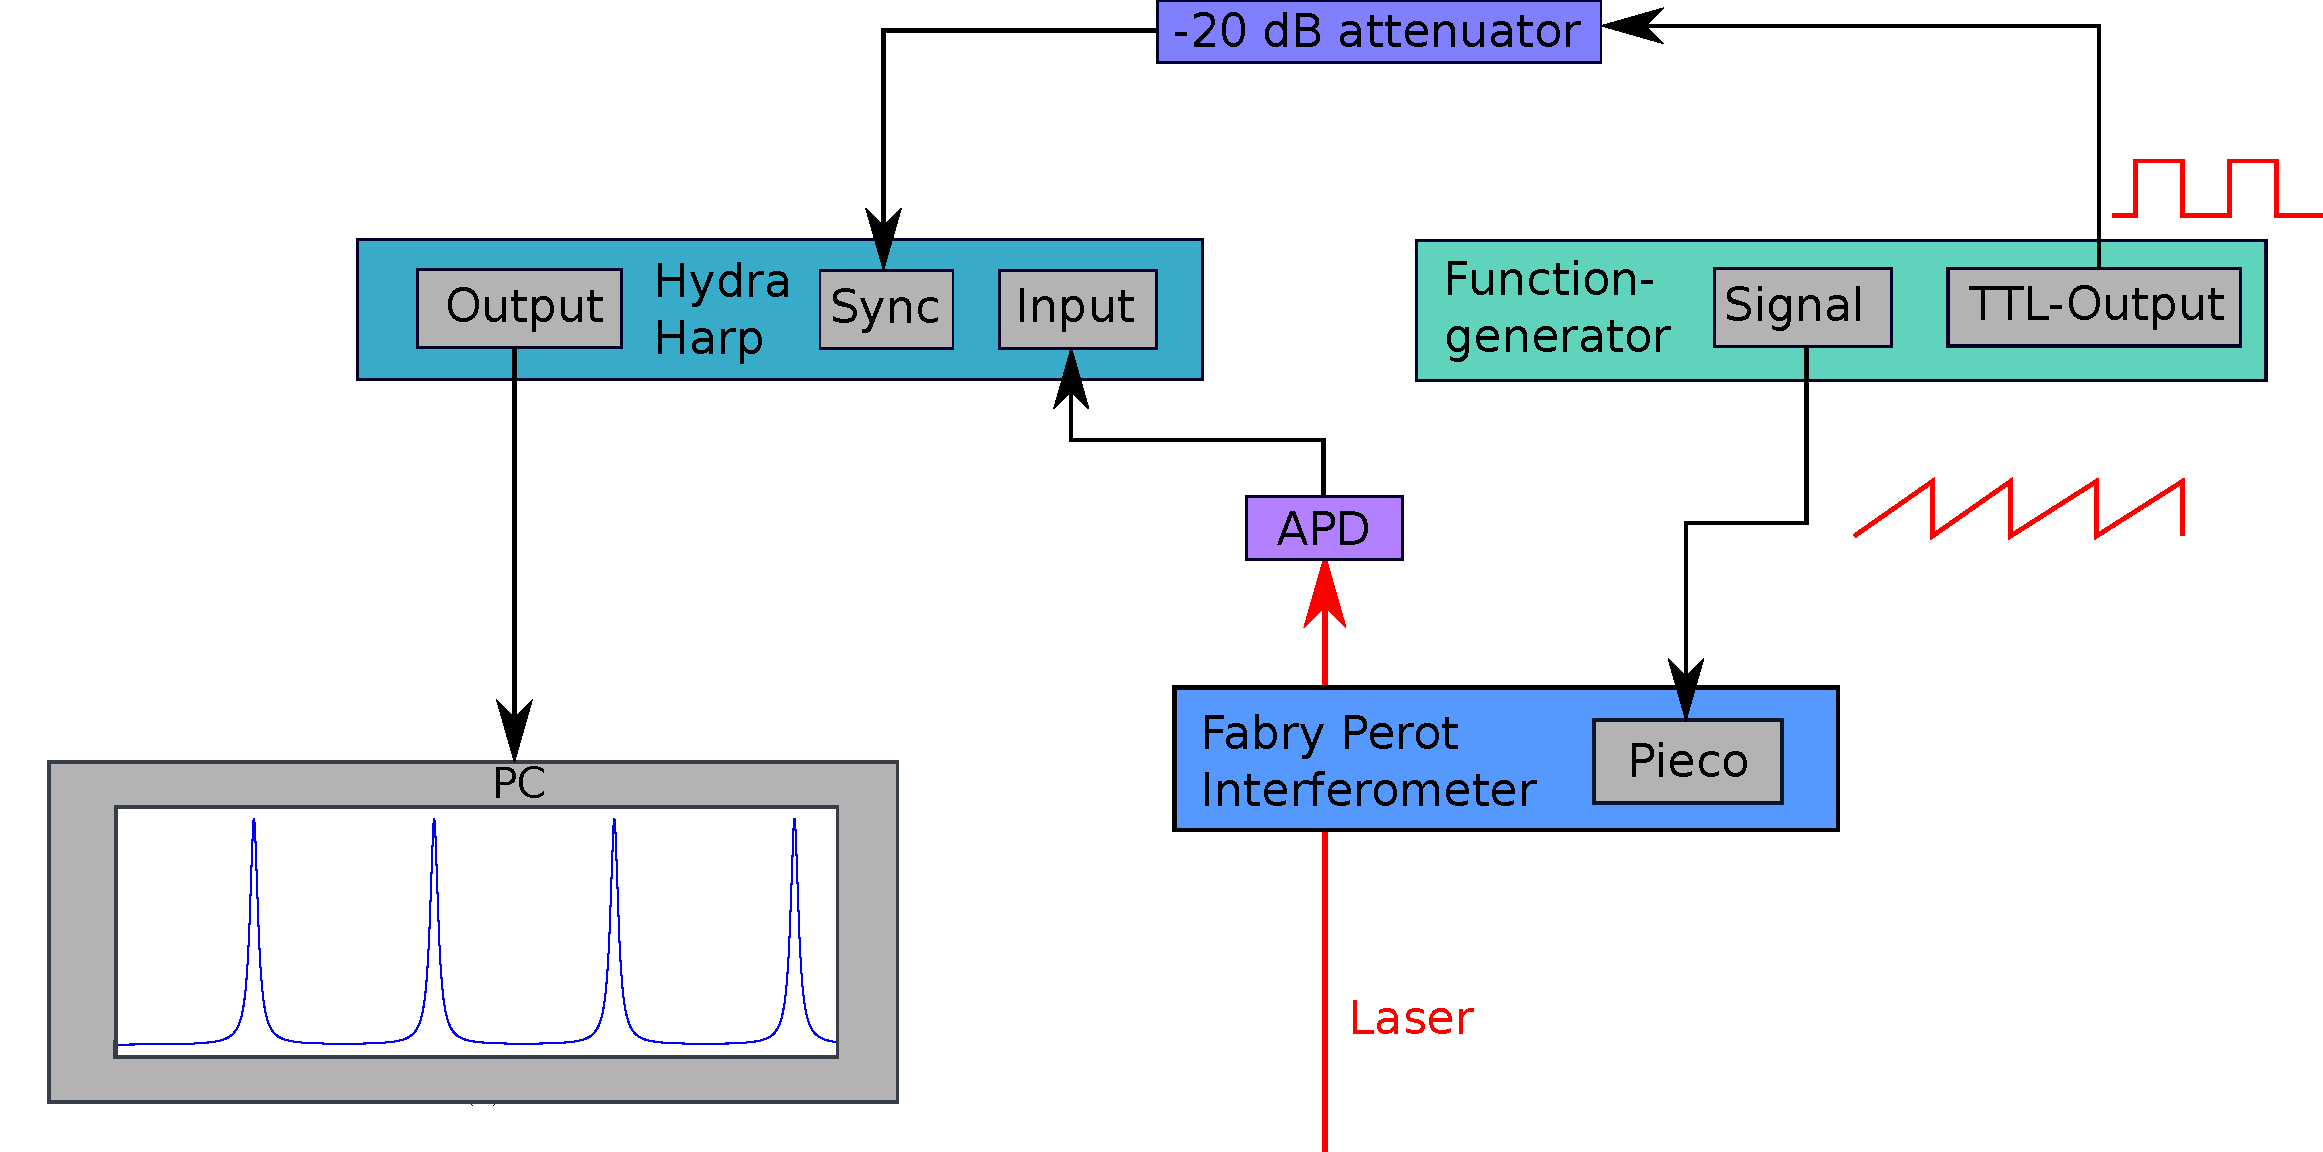
\includegraphics[width=\linewidth]{figures/fabry-perot/live-apd-setup}
	\caption{Live avalanche photodiode setup with using a function generator driving the piezo actuator of the FPI and the sync input of the correlation hardware.
	APDs are used because of their speed, allowing to live-adjusting the FPI-parameters.}
	\label{fig:live-apd-setup}
\end{figure}

Before the scanning \ac{FPI} can be used to measure \ac{QD} emission, it has to be aligned first.
\acp{APD} are used for aligning the \ac{FPI} as they are fast enough to measure the multiple free spectral ranges with a scanning frequency in the order of \si{\hertz}.
A function generator is used to drive the piezoelectrical actuator and the correlation hardware (here: Picoquant Hydraharp 400) correlates the measurements of the \ac{APD} with the TTL-output of the function generator.
The correlation hardware uses \ac{NIM} as input, while the TTL-output uses \ac{BNC}.
Because of that a \ac{NIM}-\ac{BNC} converter had to be used in between.
The complete setup is sketched in figure~\ref{fig:live-apd-setup}.

Figure~\ref{fig:2019-03-1914-10fabry-perot-live-apdrealigned} shows the measurement of the scanning \ac{FPI} with the \acp{APD}.
The scanning frequency is \SI{5}{\hertz} and the range is \SI{1}{\micro \meter}.
The measured finesse is $\approx 5$ and the free spectral range corresponds to \SI{280}{\nano \meter}.
The stability for one snapshot as visible here appears good, however the modes shift visibly over a longer period of time.


\begin{figure}[H]
	\centering
	\includegraphics[width=\linewidth]{figures/fabry-perot/plots/2019-03-19_14-10_Fabry-Perot-Live-APD_realigned}
	\caption{Measurement of scanning FPI with APDs.
	         The scanning frequency is \SI{5}{\hertz} and the range is \SI{1}{\micro \meter}.
             The measured finesse is $\approx 5$ and the free spectral range corresponds to \SI{280}{\nano \meter}.}
	\label{fig:2019-03-1914-10fabry-perot-live-apdrealigned}
\end{figure}

\subsection{Scanning mode with CCD}

In order to obtain the spectral emission of the input signal, the \ac{FPI} is used in the scanning mode.
Here one of the mirrors is attached to a piezoelectric actuator which moves the mirror stepwise after every measurement as shown in figure~\ref{fig:setup}. A minimal sketch of the setup is visible in figure~\ref{fig:setupflat}.
\begin{figure}[H]
	\centering
	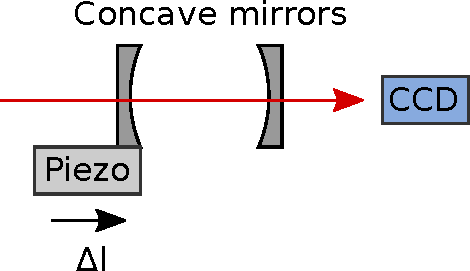
\includegraphics[width=0.4\linewidth]{figures/fabry-perot/setup/setup}
	\caption{Scanning Fabry Pérot interferometer}
	\label{fig:setup}
\end{figure}




\section{Measurements and discussion}
\label{sec:fabry-measurements}

In the following measurements the \ac{FPI} was set up in the non-confocal mode and HeNe laser signals were used in order to align it.
This involves for one setting the mirrors coming before the \ac{FPI} so that the laser beam goes straight and centred through the \ac{FPI} mirrors and then setting the \ac{FPI} mirrors so that they are parallel and a single laser beam emerges as is shown in figure~\ref{fig:align-fpi}.


\begin{figure}[H]
	\centering
	\begin{subfigure}[b]{0.48\textwidth}
		\centering
		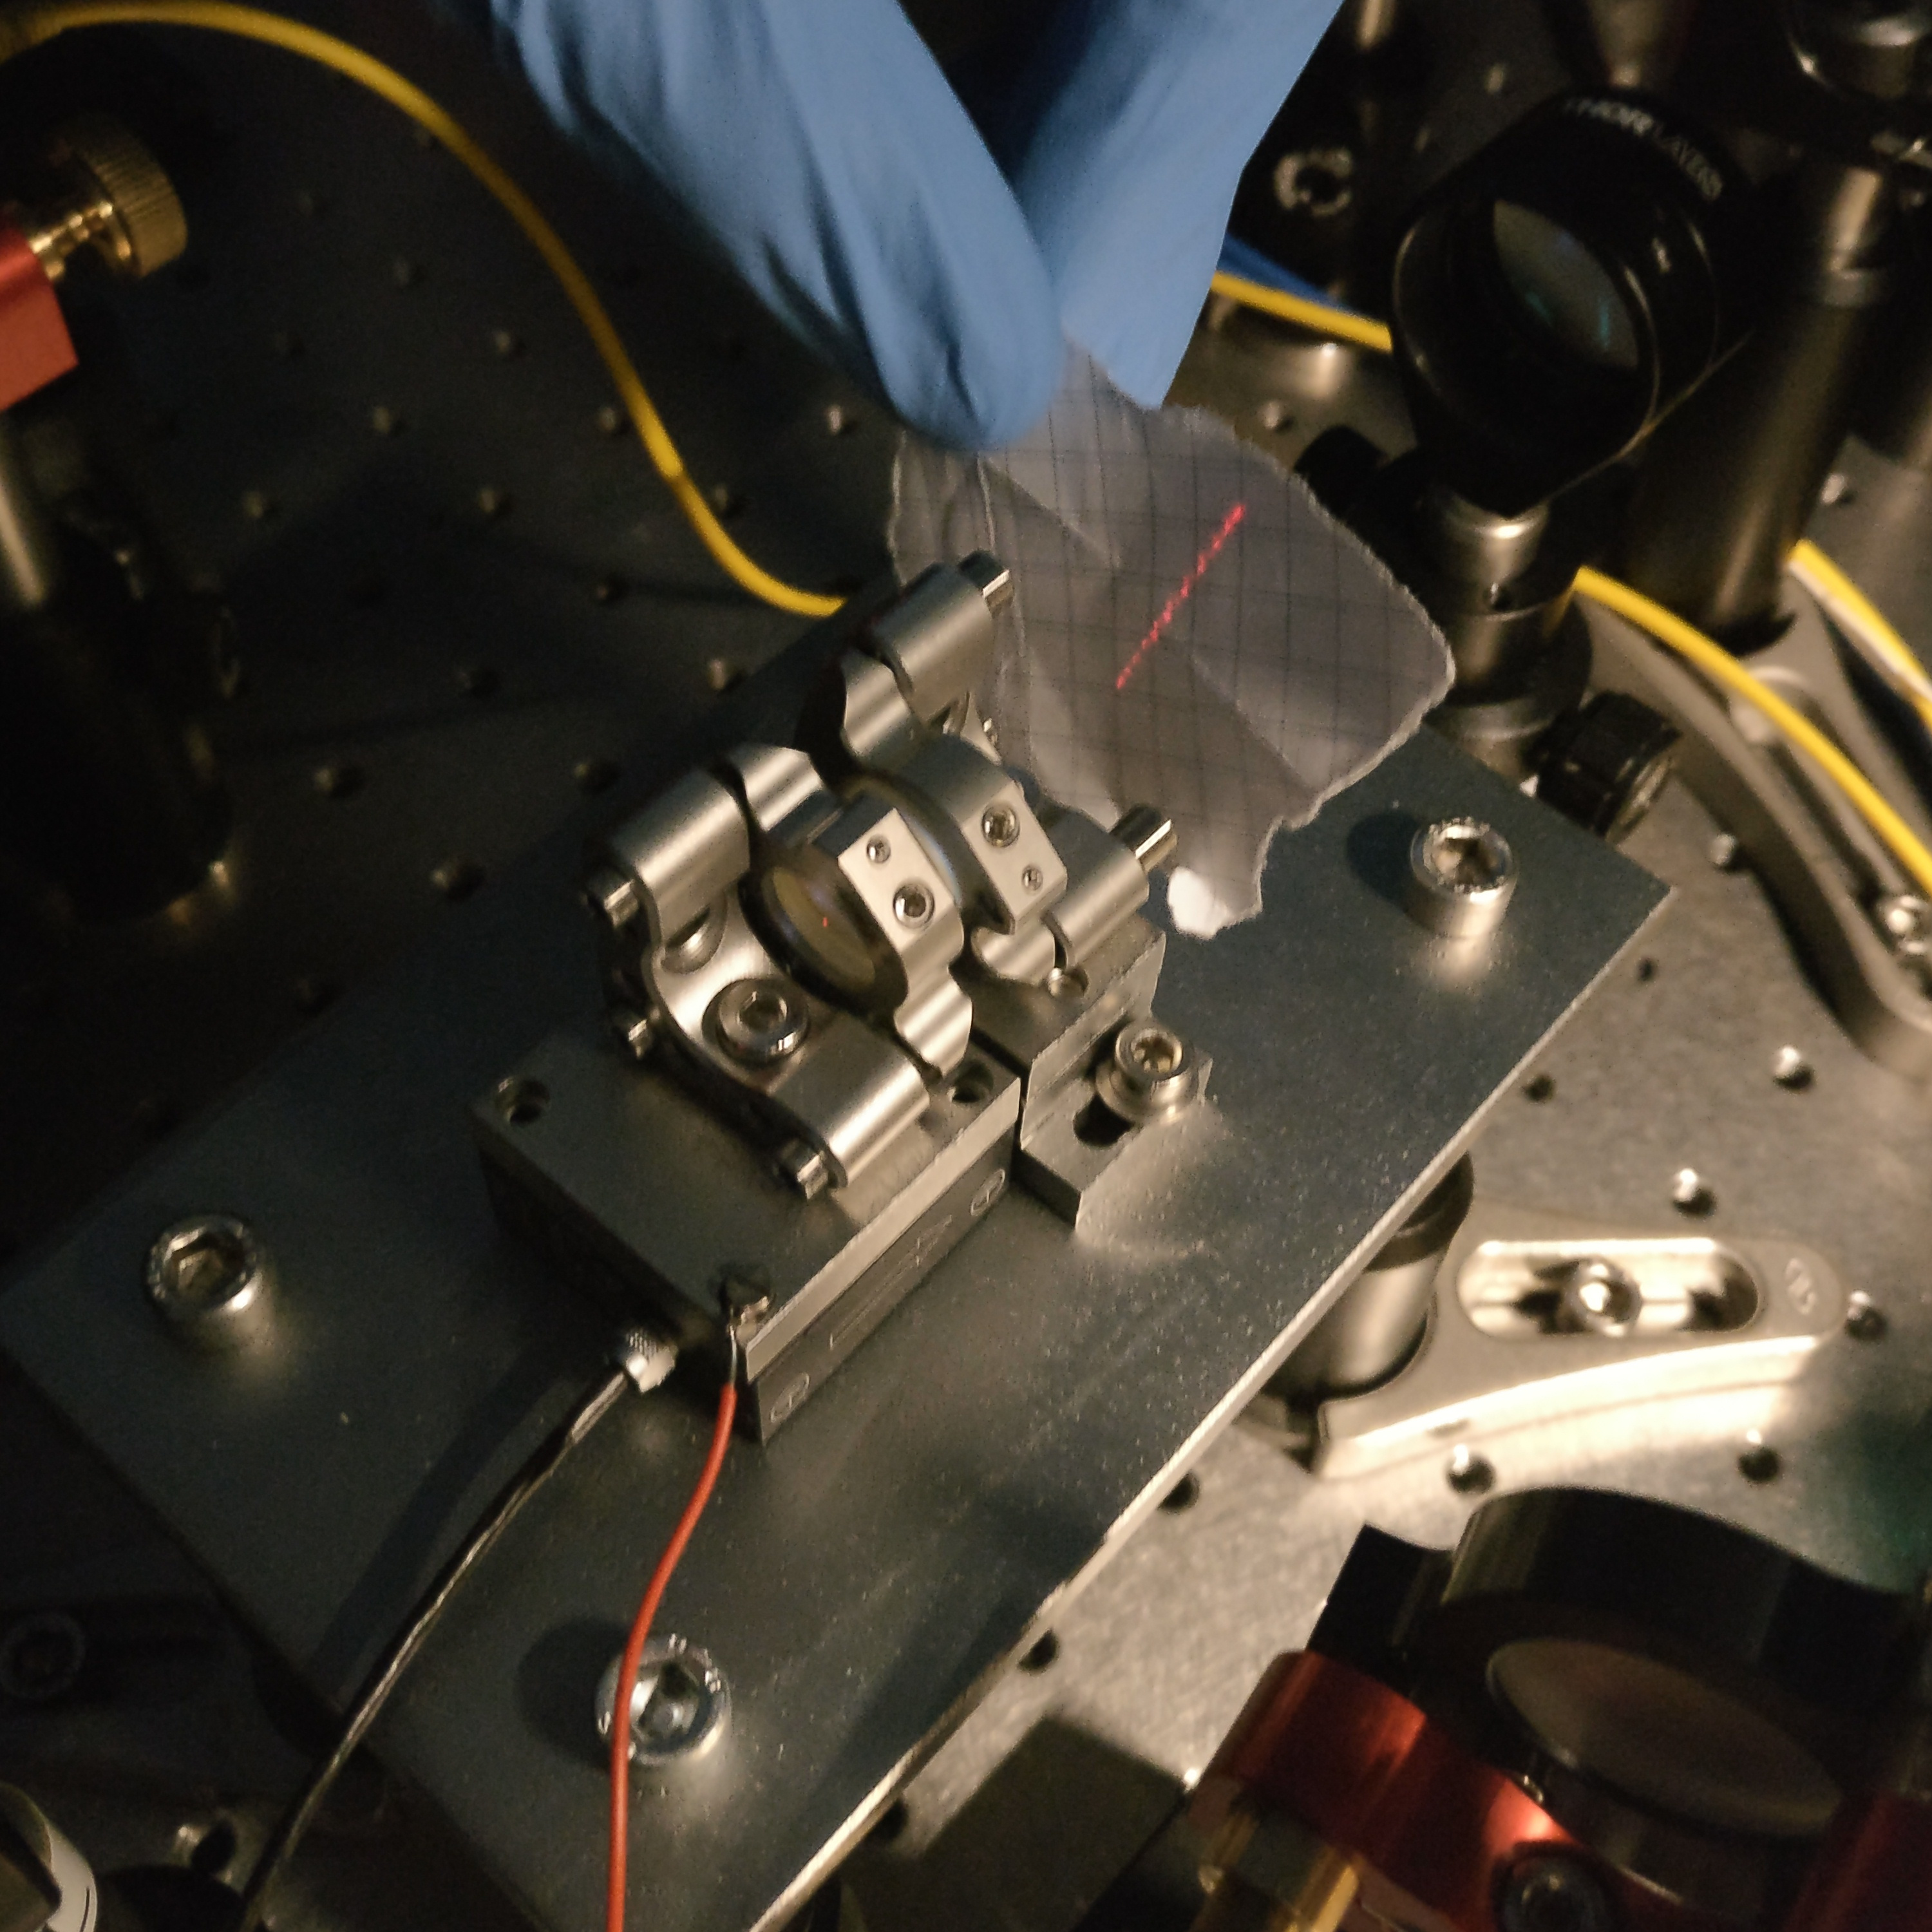
\includegraphics[width=0.95\textwidth]{figures/fabry-perot/setup/confocal-setup-higher-modes-1}
		\caption{}
		\label{fig:confocal-setup-higher-modes-1}
	\end{subfigure}%
	~ % An dieser Stelle kann ein zusätzlicher Zwischenraum eingebunden werden: ~, \quad, \qquad, \hfill usw.
	% Eine leere Zeile erzwingt, dass die zweite Grafik darunter erscheint.
	\begin{subfigure}[b]{0.48\textwidth}
		\centering
		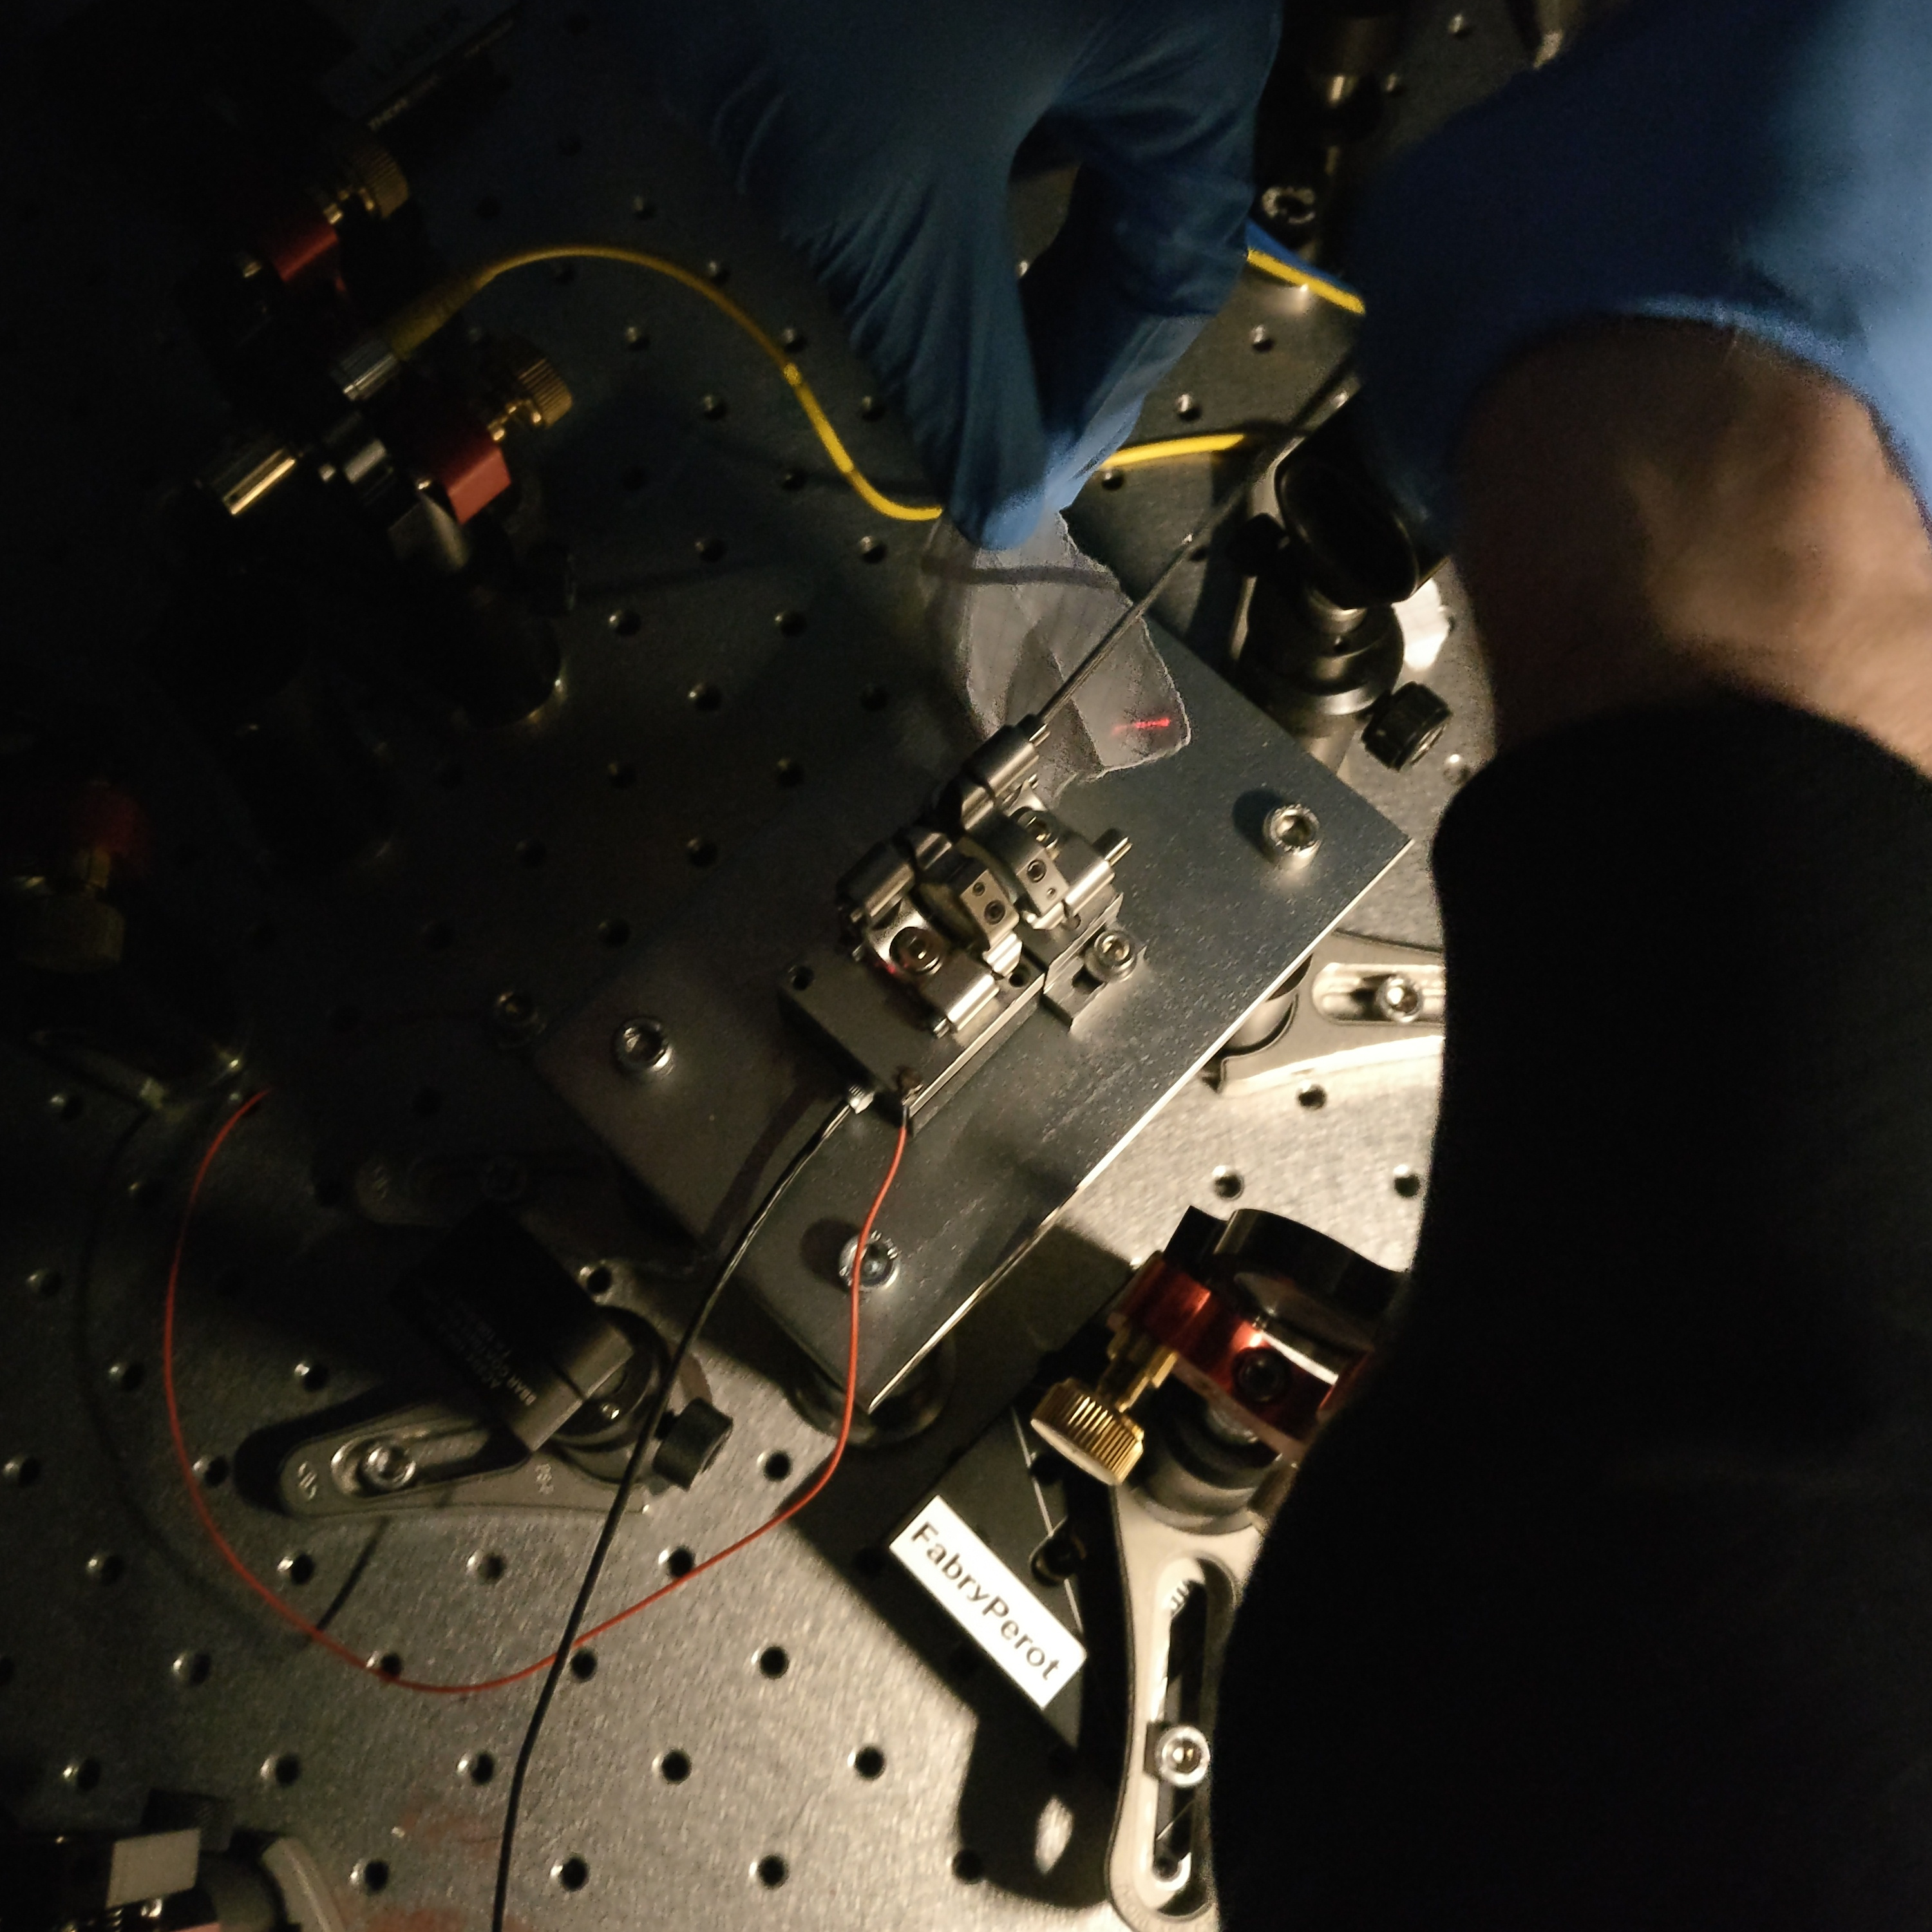
\includegraphics[width=0.95\textwidth]{figures/fabry-perot/setup/confocal-setup-higher-modes-2}
		\caption{}
		\label{fig:confocal-setup-higher-modes-2}
	\end{subfigure}
	\caption{Aligning the Fabry Pérot interferometer}
	\label{fig:align-fpi}
\end{figure}

Without spatial restriction strong TEM-modes of higher order are visible in figure~\ref{fig:measurement-fabry-perot-hene}(a).
To counteract, a pinhole is inserted and adjusted which results in the measurement visible in figure~\ref{fig:measurement-fabry-perot-hene}(b).

\begin{figure}[H]
	\centering
	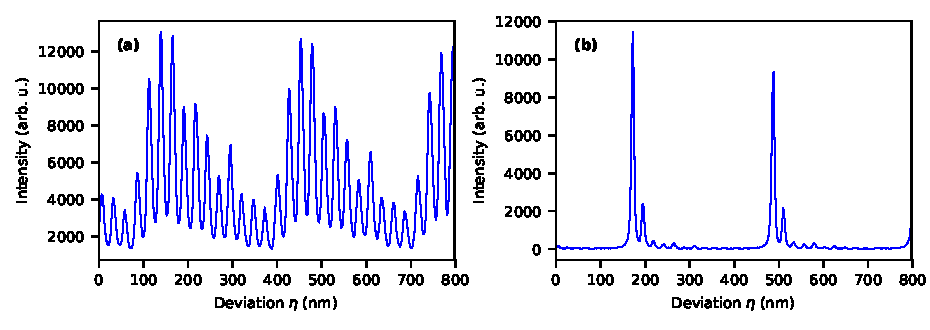
\includegraphics[width=\linewidth]{figures/fabry-perot/plots/measurement-fabry-perot-HeNe}
	\caption{Transmission measurement of FPI with ground mirror distance $l \approx \SI{2}{\milli \meter}$ and HeNe laser. (a) was aligned without spatial filtering with a pinhole and (b) involved a pinhole.}
	\label{fig:measurement-fabry-perot-hene}
\end{figure}

Set up like this, the GaAs \ac{QD} sample AS208 was measured.
First a polarization map of the exciton was recorded in order to determine the \ac{FSS} $E_{FSS}=\SI{24.42 (39)}{\micro \electronvolt}$ with the data shown in figure~\ref{fig:measurement-fabry-perot-dot-exciton-pol-map}.
\todo{how does this work. Explain more details, this is not trivial}

\begin{figure}[H]
	\centering
	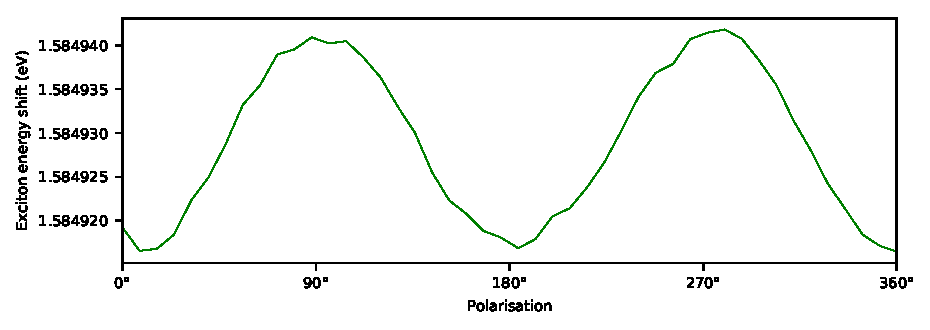
\includegraphics[width=\linewidth]{figures/fabry-perot/plots/measurement-fabry-perot-dot-exciton-pol-map}
	\caption{Polarization map of exciton of QD in sample AS208.}
	\label{fig:measurement-fabry-perot-dot-exciton-pol-map}
\end{figure}

Afterwards the output of the \ac{QD} through the \ac{FPI} was measured while the mirror distance was stepwisely changed which is shown in figure~\ref{fig:measurement-fabry-perot-dot-biexciton-fss}.
The x-scale on the top of figure~\ref{fig:measurement-fabry-perot-dot-biexciton-fss} was calculated by correlating the distance between the two adjacent peaks with the \ac{FSS} determined with the data of figure~\ref{fig:measurement-fabry-perot-dot-exciton-pol-map}.
For this \ac{QD} results in a conversion between the deviations $\eta=\SI{1}{\nano \meter} \equalhat \zeta = \SI{1.19 (2)}{\micro \electronvolt}$.
\todo{What does this comparison tell us? Did it fit the calculation? Where are the side peaks we saw in the HeNe measurement? What a about the stability? Are there calculations, expected temperature drifts, etc. Are there differences between the expected Finesse and the measured one, and why? Is this expected?}


\begin{figure}[H]
	\centering
	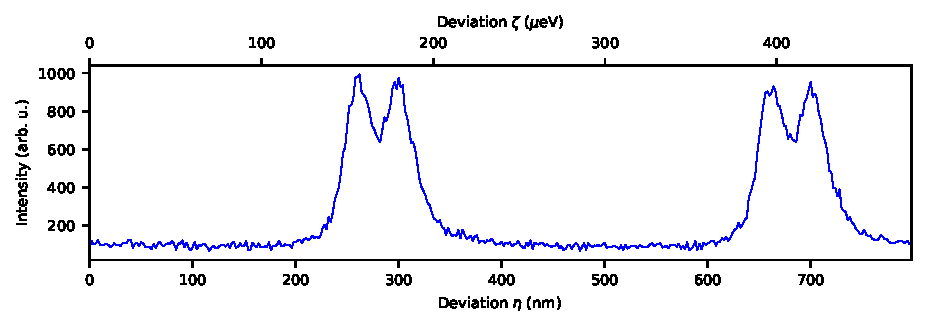
\includegraphics[width=1\linewidth]{figures/fabry-perot/plots/measurement-fabry-perot-dot-biexciton-FSS}
	\caption{Finestructure measurement of biexcition of QD in sample AS208 by passing thorugh FPI and sweeping the mirror distance.
	Ground mirror distance was  $l \approx \SI{2}{\milli \meter}$.}
	\label{fig:measurement-fabry-perot-dot-biexciton-fss}
\end{figure}




